\documentclass{ceurart}

\usepackage{acronym}
\usepackage{subcaption}

\renewcommand{\acffont}[1]{\textsl{#1}}


%%
%% end of the preamble, start of the body of the document source.
\begin{document}

%%
%% Rights management information.
%% CC-BY is default license.
\copyrightyear{2023}
\copyrightclause{Copyright for this paper by its authors.\\
  Use permitted under Creative Commons License Attribution 4.0
  International (CC BY 4.0).}

%%
%% This command is for the conference information
\conference{CLEF 2023: Conference and Labs of the Evaluation Forum, September 18--21, 2023, Thessaloniki, Greece}

%%
%% The "title" command
\title{SEUPD@CLEF: Team <Acronym> on <Short Description>}

\title[mode=sub]{Notebook for the LongEval Lab at CLEF 2023}

%%
%% The "author" command and its associated commands are used to define
%% the authors and their affiliations.
\author[1]{Name Surname}[%
email=name.surname@studenti.unipd.it
]

\author[1]{Name Surname}[%
email=name.surname@studenti.unipd.it
]

\author[1]{Name Surname}[%
email=name.surname@studenti.unipd.it
]

\author[1]{Nicola Ferro}[%
orcid=0000-0001-9219-6239,
email=ferro@dei.unipd.it,
url=http://www.dei.unipd.it/~ferro/,
]


\address[1]{University of Padua, Italy}


%%
%% The abstract is a short summary of the work to be presented in the
%% article.
\begin{abstract}
  A clear and well-documented \LaTeX{} document is presented as an
  article formatted for publication by CEUR-WS in a conference
  proceedings. Based on the ``ceurart'' document class, this article
  presents and explains many of the common variations, as well as many
  of the formatting elements an author may use in the preparation of
  the documentation of their work.
\end{abstract}

%%
%% Keywords. The author(s) should pick words that accurately describe
%% the work being presented. Separate the keywords with commas.
\begin{keywords}
  keyword 1 \sep
  keyword 2 \sep
  keyword 3 
\end{keywords}

%%
%% This command processes the author and affiliation and title
%% information and builds the first part of the formatted document.
\maketitle


\section{Introduction}
\label{sec:introduction}

Introduce the context, motivations, and goals of your project.

The paper is organized as follows: Section~\ref{sec:methodology} describes our approach; Section~\ref{sec:setup} explains our experimental setup; Section~\ref{sec:results} discusses our main findings; finally, Section~\ref{sec:conclusion} draws some conclusions and outlooks for future work.

\section{Related Work}
\label{sec:related}

Describe related works, i.e. previous approaches to solve your problem you have started or improved from.

\section{Methodology}
\label{sec:methodology}

%Describe the methodology you have adopted, the %architecture of your system, your workflow, etc.
%Nostra metodologia: "miglioramento continuo", integrazione in base all'andamento delle metriche di prestazione. (Sommariamente, azioni? configurazione Filter, filtraggio documenti, tecniche nlp ecc.?)
%Quali metriche abbiamo preso per riferimento (presenti in treceval), strumenti e tecniche per evidenziare i problemi (es. citazione a tellme.c).
%Presenza dei diversi branch per evidenziare i flussi di lavoro paralleli per le diverse lingue.

In the roadmap of this project, the first goal we intended to achieve was to reach a stable and simple version of a basic indexing and searching system, to be used as a baseline to experiment additional features on. 
\par
Afterwards, the workflow split into several lines, each applying a different improvement strategy, such as different analyzing techniques, different filter configurations or different document preprocessing operations. Once a better system was found, it would eventually become the new baseline to run further experiments on.
In order to operate in this way, each line would evolve on a different working branch of our git repository, with its performance measured mainly through trec\_eval's nDCG and/or MAP metric.
\par
Some tools were also developed to help us analyze what kind of errors the run contained, to perform some pre-processing to the collection documents and to solve some translation problems.
\par
The main programming language that we used to develop our systems is Java, while some tools have been developed using Python. In particular, the core of our work was implemented by exploiting the Lucene java library \cite{lucene}.
\par
We can split our systems in four main components:
\begin{itemize}
	\item \textbf{Parser}: it parses the corpus independently of the language chosen by using the TREC file format.
	\item \textbf{Analyzer}: it processes some text performing tokenization, stopword removal, stemming and other filtering processes.
	\item \textbf{Indexer}: it processes the parsed and analyzed documents fields to creates the index.
	\item \textbf{Searcher}: it processes a given query and exploits the index to retrieve some documents based on the processed query.
\end{itemize}

\par
In this section we describe the general workflow of our systems (Section \ref{subsec:genflow}), the developed tools ( Sections \ref{subsec:preprocess} and \ref{subsec:transltools}), the general components (Sections \ref{subsec:parser}, \ref{subsec:analyzer}, \ref{subsec:indexer} and \ref{subsec:searcher}) and the complete systems (Section \ref{subsec:systems}).

\subsection{General systems flow}
\label{subsec:genflow}
All of our systems operate in the following order:
\begin{enumerate}
	\item Apply a pre-processing to the documents of the corpus (optional stage).
	\item Parse the documents of the corpus, splitting the content into the appropriate fields, using the parser.
	\item Analyze the documents' fields to convert them into a stream of tokens and index them to perform the search (single index folder).
	\item Parse and analyze the queries to convert them into a stream of tokens.
	\item Perform the search by exploiting the index (one query at the time).
	\item Rerank the documents retrieved with the search (optional stage).
	\item Print the results of the search into a dedicated text file.
\end{enumerate}

\subsection{Pre-processing tools}
\label{subsec:preprocess}
\subsubsection{SPAM parser}
\label{subsubsec:spam}
By analyzing the results produced with the French-based system (the simplest one) on the French collection, we realized that relevant documents for a specific query were not included in the first one thousand documents retrieved by the system for that query. Before increasing the system's complexity through new features, while inspecting the retrieved documents, it turned out that several of them were ranked with a high score due to the high number of words repetitions. More precisely, excluding documents that were actually not relevant, we noticed that in the analyzed documents the words were not different and the text contained a sensible number of repetitions. This new information drove us to develop term frequency analyses to avoid the retrieval of documents considered "spam" during the search task or, even better, the addition to the Lucene index during the index task, reducing its overall size.  
\par
With the term "spam" we denote the type of documents that "hack" the retrieval system through the use of a set of words contained in the user query, that brings the document to the top of the document-ranked list.   
\par
The following documents are some examples of "spam". We can notice that the length of the texts is very short compared to the one of an average document: 
\begin{quote}
    \centering \textit{"\textbf{Tableau} de conversion pouce / inch en Cm mm | \textbf{Tableau} de conversion, \textbf{Tableau} de conversion de mesure, Scrapbooking à imprimer"} 
\end{quote}
\begin{quote}
    \centering  \textit{"[...] \textbf{Quiz} : Cinéma \textbf{Quiz} : Histoire de France \textbf{Quiz} : Géographie \textbf{Quiz} : Histoire \textbf{Quiz} : Littérature \textbf{Quiz} : Espace \textbf{Quiz} : Bien-être \textbf{Quiz} : Littérature \textbf{Quiz} : Gamer \textbf{Quiz} : Formule 1 \textbf{Quiz}"[...] }
\end{quote}
The methodology that we applied to fulfil this goal takes into account two main factors:  
\begin{enumerate}
    \item The ratio between the most frequent word and the total length of the document, excluding articles and stopwords: 
    \begin{equation}
        \frac{\text{Max freq}}{\text{Doc length}}.
    \end{equation} 
    The value obtained is as low as the term occurrences are spread all over the document.
    \item The ratio between the number of words in the document and the number of different words used in it:
    \begin{equation}
        \frac{\text{Doc length}}{\text{Number different words}}.
    \end{equation} This value reaches higher values for documents which contain the same few words repeated many times. For this reason, they may not contain any useful information for the user.  
\end{enumerate}
In order to combine the two approaches, we can obtain a third ratio by multiplicating the previous ones and comparing the result with a threshold:
\begin{equation}
    \frac{\text{Max freq}}{\cancel{\text{Doc length}}} \cdot \frac{\cancel{\text{Doc length}}}{\text{Number different words}} = \frac{\text{Max freq}}{\text{Number different words}} > \text{threshold}
\end{equation}
\par
During the process, one more threshold is checked: the length of the analyzed word. Since the implemented parser splits the sentences using blank spaces, it may happen that sequence of characters (e.g. "$\star \star \star$", "NVO",..) or symbols (e.g. €) cause an erroneous document exclusion. By applying the proposed threshold these errors are avoided. 
\par
The entire pre-processing task was implemented in a separate Python file which automatically reads all the files in the French collection and for each file it saves a new one that doesn't contain the documents marked as spam. The overall flow is reported in Figure\ref{fig:doc_parser-figure}. 

\begin{figure}
  \centering
  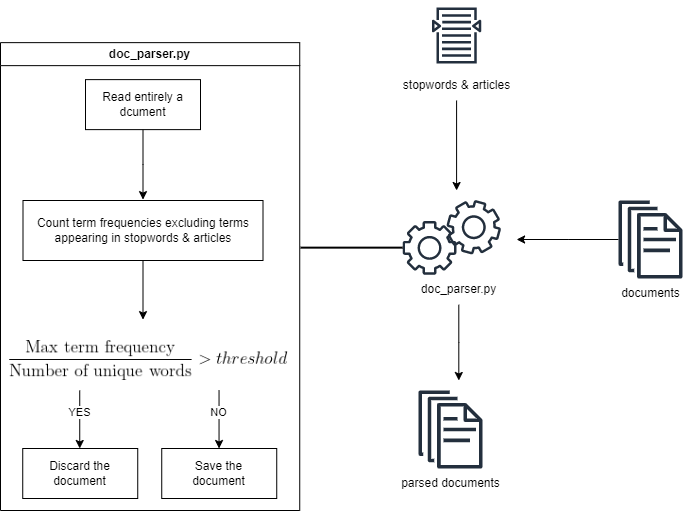
\includegraphics[width=250px,scale=0.5]{figure/doc_parser-diagram.png}
  \caption{Flow of the documents parser. (\href{https://bitbucket.org/upd-dei-stud-prj/seupd2223-dards/src/french/docs_filter.py}{docs\_filter.py}).}
  \label{fig:doc_parser-figure}
\end{figure}

\subsubsection{Synonyms}
\label{subsubsection:synonyms}
In order to try to increase the system's performance, a query expansion method was implemented through the use of synonyms. The files containing French synonyms available on the internet were not sufficient and covered only a small part of the entire French dictionary. For this reason, a new collection of words that could be easily used as synonyms of words found in the queries during the search task was needed. To address this need, another Python tool that automatically performs a request to a specialized site \url(dictionary.reverso.net/french-synonyms/) and retrieves all the related synonyms was created. All the new words found are placed in the same line as the searched word so that the Searcher (\ref{subsec:searcher}) can easily extract the information needed. The overall flow is shown in Figure \ref{fig:search_synonyms-figure}.

\begin{figure}
  \centering
  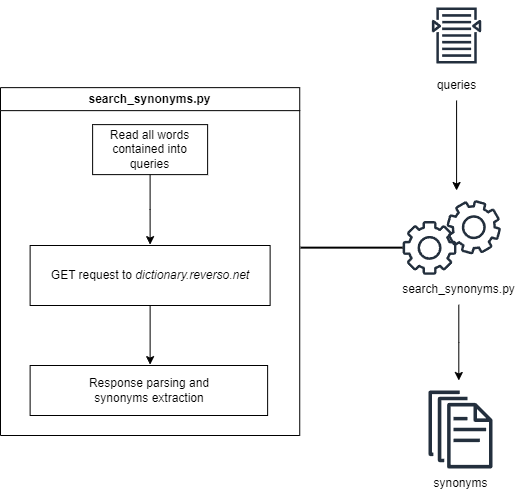
\includegraphics[width=250px,scale=0.5]{figure/search_synonyms.png}
  \caption{Flow of the synonyms searcher. (\href{https://bitbucket.org/upd-dei-stud-prj/seupd2223-dards/src/french/search_synonyms.py}{search\_synoyms.py}).}
  \centering \label{fig:search_synonyms-figure}
\end{figure}


\subsection{Translation tool}
\label{subsec:transltools}
Since the translations of the documents and the queries provided by CLEF resulted to be imprecise, we developed a tool that allows to translate a piece of text from French to English.
The tool has been implemented as a script in Google's "Google App Script" platform and then deployed as a web application. This tool must be used as a REST resource.
\par
The code used to implement this tool can be found \href{https://bitbucket.org/upd-dei-stud-prj/seupd2223-dards/src/master/code/BM25TRANSLATEDQUERIES/src/main/java/it/unipd/dei/dards/utils/GoogleScriptApi.gs}{HERE}.

\subsection{Parser}
\label{subsec:parser}
The parser that we implemented for all of our systems is a basic parser. This component simply reads all the files with a given extension (.txt) present in a directory tree (specified as input) and converts all the \textbf{Trec} formatted documents into an instance of document that has two fields: the identifier of the document (ID) and the body of the document (BODY). Some systems in addition to that also read another file (whose path is given as input) that contains pairs "document identifier"-"document url" and add an additional url field (URL) to the instances of the documents based on the identifier. In some systems, we decided to add this field for two reasons: the URL could help decreasing the rank position of the document containing "spam" (see section \ref{subsec:preprocess}) and it could help us in the queries that contain a website url.
\par
Furthermore, we tried also to add another field to the document instances that was meant to contain the document keywords (retrieved exploiting an algorithm called RAKE \cite{rake}, Rapid Automatic Keyword Extraction), but it required too much computation time so we didn't implement this option.
\par
Eventually, the parsing of the queries uses the \textbf{tsv} file format and it is done in the searcher module (see Section \ref{subsec:searcher}).

\subsection{Analyzer}
\label{subsec:analyzer}
In our systems we implemented customized analyzers instead of using the standard ones proposed by Lucene. This choice was motivated by the fact that this way we could customize the filters pipeline and choose a tokenizer. Tokenizers process the input stream (the document text) and using some predefined rules they split it into tokens: these are the atomic units composing a document. Unlike words, tokens do not have to be grammatically correct or meaningful, but are suitable for processing and comparison operations.
We tried two different tokenizers:
\begin{itemize}
    \item \textbf{StandardTokenizer}: a grammar-based tokenizer constructed with JFlex. It implements the Word Break rules from the Unicode Text Segmentation algorithm, as specified in Unicode Standard Annex \#29.
    \item \textbf{WhiteSpaceTokenizer}: it breaks text into terms whenever it encounters a whitespace character.
\end{itemize}
We started out using StandardTokenizer and we noticed that expressions separated with hyphens were divided into different tokens. To avoid this, we tried a combination of WhiteSpaceTokenizer and PatternReplaceFilter to remove all punctuations/symbols except for hyphens. But then performances decreased and we backtracked.
\\
In addition to the StandardTokenizer we used different filters, some of them shared by both English-based and French-based systems:
\\
\textbf{French}
\begin{itemize}
    \item \textbf{ElisionFilter}: it targets elisions, so removes articles, prepositions and conjunctions placed either in the initial or final part of the token, usually connected by an apostrophe or hyphen. This connection makes it impossible for a generic stopword filter alone to detect and delete those particles.
    \item \textbf{ASCIIFoldingFilter}: it converts alphabetic, numeric, and symbolic Unicode characters which are not in the Basic Latin Unicode block (the first 127 ASCII characters) to their ASCII equivalents, if one exists. This filter was used to solve accents and diacritical marks problem with French.
    \item \textbf{FrenchLightStemFilter}: this stemmer implements the "UniNE" algorithm \cite{frenchlightstemmer}.
\end{itemize}
Note that for the French case other stemmers (FrenchMinimalStemmer, org.taurus.snowball's FrenchStemmer) and combination of stemmers have been tested and evaluated but the performances of the FrenchLigthStemmer turned out to be the best.
\\
\textbf{English}
\begin{itemize}
    \item \textbf{NGramFilter}: it generates n-gram tokens of sizes in the given range. Tokens are ordered by position and then by gram size.
    \item \textbf{ShingleFilter}: it constructs shingles, which are token n-grams, from the token stream. it combines runs of tokens into a single token.
    \item \textbf{PorterStemFilter}: it applies the Porter Stemming Algorithm for English. The results are similar to using the Snowball Porter Stemmer with the language="English" argument. It is coded directly in Java and it is four times faster than the English Snowball stemmer.
    \item \textbf{KStemFilter}: it is an alternative to the Porter Stem Filter for developers looking for a less aggressive stemmer. KStem was written by Bob Krovetz, ported to Lucene by Sergio Guzman-Lara (UMASS Amherst). This stemmer is only appropriate for English language text.
\end{itemize}

\textbf{Shared}
\begin{itemize}
    \item \textbf{LowerCaseFilter}: it converts any uppercase letter in a token to the equivalent lowercase token. All other characters are left unchanged.
    \item \textbf{StopFilter}: it discards, or stops analysis of, tokens that are on the given stop words list.
    \item \textbf{SynonymGraphFilter}: it maps single- or multi-token synonyms, producing a fully correct graph output. If used for indexing it must be followed by a FlattenGraphFilter to squash tokens on top of one another, because the indexer can’t directly consume a graph.
    \item \textbf{HyphenatedWordsFilter}: it reconstructs hyphenated words that have been tokenized as two tokens because of a line break or other intervening whitespace in the field test. If a token ends with a hyphen, it is joined with the following token and the hyphen is discarded.
    \item \textbf{RemoveDuplicatesTokenFilter}: it removes duplicate tokens in the stream. Tokens are considered to be duplicates ONLY if they have the same text and position values.
    \item \textbf{NumberFilter}: it removes every token in the token stream that happens to be a number (this filter has been developed by team DARDS).
\end{itemize}

\subsection{Indexer}
\label{subsec:indexer}
The indexer's job is to store the tokens, generated by processing every document with a given analyzer, into an inverted index (data structure which maps terms to documents).
We implemented two types of indexer, \textit{DirectoryIndexer} and \textit{ReRankDirectoryIndexer}, the first one takes all the documents in a given directory and stores them into the index, the second one does the same but it can also store a list of documents passed to it.
\\
Lucene captures some statistics at indexing time which can then be used to support scoring at query time. To do this it makes use of similarity functions, which set a per-document value for every field in the document. Hence, the similarity determines how Lucene weights terms.
\\
In our systems we tested different similarities:

\begin{itemize}
    \item \textbf{BM25Similarity}: it implements the Okapi BM25 (Best Match, attempt 25).
    \item \textbf{LMDirichletSimilarity}: bayesian smoothing using Dirichlet priors. The formula assigns a negative score to documents that contain the term, but with fewer occurrences than predicted by the collection language model.
    \item \textbf{LMJelinekMercerSimilarity}: language model based on the Jelinek-Mercer smoothing method. The model has a single parameter, $\lambda$. The optimal value is around 0.1 for title queries and 0.7 for long queries. Values near zero act score more like a conjunction (coordinate level matching), whereas values near 1 behave the opposite (more like pure disjunction).
    \item \textbf{DFRSimilarity}: it implements the divergence from randomness (DFR) framework. Probabilistic models of IR based on measuring the divergence from randomness. The DFR scoring formula is composed of three separate components: the basic model, the aftereffect and an additional normalization component.
    \item \textbf{ClassicSimilarity}: subclass of TFIDFSimilarity. Lucene combines Boolean model (BM) of Information Retrieval with Vector Space Model (VSM) of Information Retrieval. In VSM, documents and queries are represented as weighted vectors in a multi-dimensional space, where each distinct index term is a dimension, and weights are Tf-idf values. VSM score of document d for query q is the Cosine Similarity of the weighted query vectors V(q) and V(d).
    \item \textbf{BooleanSimilarity}: it gives terms a score that is equal to their query boost.
    \item \textbf{AxiomaticF2LOG}: it is defined as $ \sum tfln(\textup{term\_doc\_freq}, \textup{docLen}) \times \textup{IDF(term)}$ whit $\textup{IDF(term)}=ln \left(\frac{N+1}{df(t)}\right)$; where $N$ equals total number of docs, $df$ corresponds to the docs frequency.
    \item \textbf{AxiomaticF2EXP}: it is defined as $ \sum tfln(\textup{term\_doc\_freq}, \textup{docLen}) \times \textup{IDF(term)}$ whit $\textup{IDF(term)}= \left({\frac{N+1}{df(t)}}\right)^k$; where $N$ equals total number of docs, $df$ corresponds to the docs frequency.
    \item \textbf{IndriDirichletSimilarity}: bayesian smoothing using Dirichlet priors as implemented in the Indri Search engine. A larger value for parameter $\mu$ produces more smoothing. Smoothing is most important for short documents where the probabilities are more granular.
    \item \textbf{MultiSimilarity}: particular similarity which implements CombSUM method for combining evidence from multiple similarity values \cite{multisim}.
\end{itemize}
In the large majority of cases the BM25Similarity turned out to be the best option to use (see Table \ref{tab:similcomp}. Note that the values of the following table refer to an initial system that performed the search on the English corpus provided by CLEF).
\begin{center}
\begin{table}[h!]
\centering
\begin{tabular}{|l|c|} 
 \hline
    \textbf{Similarity} &  \textbf{MAP}  \\
 \hline\hline
 BM25Similarity & 0.1424  \\ 
 LMJelinekMercerSimilarity(0.1F) & 0.1249   \\
 LMJelinekMercerSimilarity(0.5F) & 0.1255  \\
 LMJelinekMercerSimilarity(0.8F) & 0.1242  \\ 
 DFRSimilarity (most of the configurations)& 0.1423\\
 LMDirichletSimilarity & 0.1204\\
 IndriDirichletSimilarity & 0.0137 \\
 ClassicSimilarity & 0.0740\\
 BooleanSimilarity & 0.0121 \\
 AxiomaticF2LOG & 0.1358 \\
 AxiomaticF2EXP & 0.1346\\
 \hline
\end{tabular}
\caption{Comparison of rerank performances.}
\label{tab:similcomp}
\end{table}
\end{center}

\subsection{Searcher}
\label{subsec:searcher}
The searcher is the other fundamental part of any IR system besides the Indexer. This component takes care of doing the matching between a document and a topic, giving as a result a ranking, which marks how relevant a document should be for a certain topic. In our application, topics are real user queries.
\par
In our systems, the searcher have been customized to first parse the queries from a provided, .tsv formatted file. Then, one query at the time, this component turns the query into a stream of tokens (exploiting a query parser and an analyzer which must be the same used for indexing), converts it into a Lucene Query and searches the index for it. After performing the actual search this tool optionally executes a rerank (see Section \ref{subsub:rerank}) and then prints the results of the overall process into a file.
\par
Note that in some systems the query is not directly turned into a Lucene Query but in the process the terms are boosted (see Section \ref{subsub:boost}). Furthermore, in the majority of cases the query is performed by considering the BODY field of the document but in some systems the same query is applied also to the URL field.

\subsubsection{Boosting}
\label{subsub:boost}
In some of our systems we decided to not to use a plain query but to boost the term according to some statistics. In particular, we computed a boost factor based on a measure that is quite similar to the the TF-IDF weight. The equations used to compute the boost factor for the term \textit{i} are the following:
\begin{equation}
 w_i={\left(\frac{ttf_i}{\sum_{j} ttf_j}\right)}^{0.2} \cdot \left(1+\log \frac{N+1}{n_i+1} \right),
\end{equation}
where with $ttf_i$ we indicate the "total term frequency" (number of occurrences of the term in the entire corpus), with $N$ the number of documents in the corpus and with $n_i$ we denote the number of documents containing the term.

\par
In order to boost the query terms we:
\begin{enumerate}
    \item Compute from the index an hash map that contains as keys the terms and as values the related weight.
    \item Get (exploiting the analyzer), from the original text of the query, the list of terms that will compose our Lucene Query.
    \item Create a TermQuery for each of the term.
    \item Wrap the TermQuery in a BoostQuery, setting the boost based on the hash map (the boost is set to zero if the term doesn't appear in the index).
    \item Merge all the BoostQuery(ies) in a BooleanQuery.
\end{enumerate}



\subsubsection{Reranking}
\label{subsub:rerank}
%Descrizione in breve: cos'è, cosa fa, a cosa serve. Effetto in generale (risultati descritti su sistema relativo).
After the searcher performed the task, some systems execute a rerank. To implement the reranking we simply consider the document retrieved by the search (hits), we create a new index based only on those documents (or only on the top-N document retrieved) and eventually we repeat the same or a slightly modified query (depending on the system) on the new index.


\subsection{Systems}
\label{subsec:systems}
In this subsection we describe the systems that we implemented. The overall system sequence diagram is reported in Figure \ref{fig:overallsys}.

\begin{figure}[h]
    \centering
    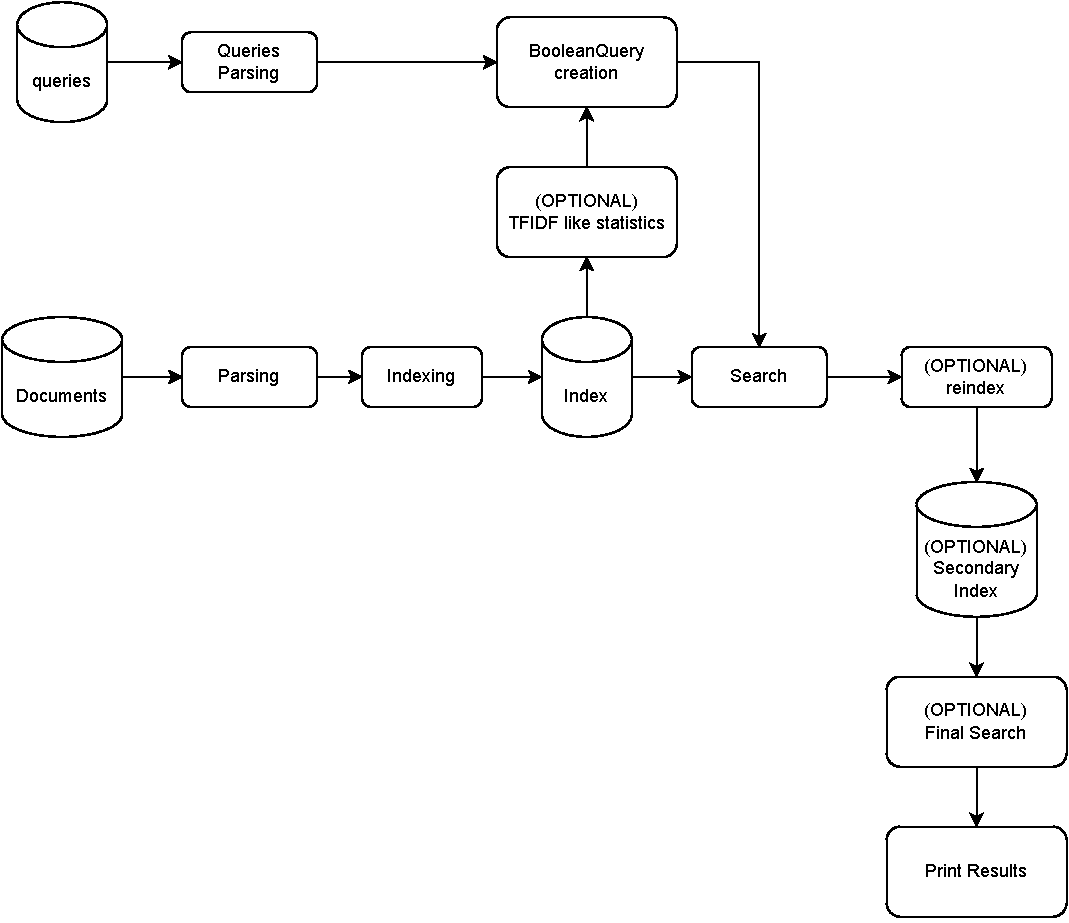
\includegraphics[scale=0.8]{figure/overallsystem.pdf}
    \caption{General system scheme}
    \label{fig:overallsys}
\end{figure}

\subsubsection{BM25FRENCHBASE system}
\label{subsub:BM25FRENCHBASE}
As a baseline for all our work, this IR system for French uses:
\begin{table}[h!]
    \centering
    \begin{tabular}{l p{0.8\linewidth}}
    Query language & French\\
    Document language & French\\
    Preprocessing & None\\
    Similarity & BM25Similarity\\
    Analyzer & Custom, composed as below\\
    Tokenizer & StandardTokenizer\\
    Filters & ElisionFilter, LowerCaseFilter, StopFilter, ASCIIFoldingFilter, FrenchLightStemFilter\\
    Searcher & Standard searcher
    \end{tabular}
\end{table}
\par This configuration has been achieved by trying all possible filter configurations while retaining only the better performing ones.
\\
The stoplist used by the StopFilter is a custom stoplist created by merging different French stoplist found online and by adding some terms based on the index created (that has been analyzed using Luke).
\\ 
The article's list used by the ElisionFilter is a custom list of terms that we created on the basis of French dictionaries. 
\\
The ASCIIFoldingFilter was used to avoid problems related to French diacritical marks and accents since not in all queries and/or documents were used properly.
\par
This system has overall good performance on the test data, especially considering its moderate complexity.

\subsubsection{BM25FRENCHBOOSTURL system}
\label{subsub:BM25FRENCHBOOSTURL}
The BM25FRENCHBOOSTURL system considers a document with three fields: ID,BODY,URL (see Section \ref{subsec:parser}). Furthermore this system uses:
\begin{table}[h!]
    \centering
    \begin{tabular}{l p{0.8\linewidth}}
    Query language & French\\
    Document language & French\\
    Preprocessing & None\\
    Similarity & BM25Similarity\\
    Analyzer & Custom, composed as below\\
    Tokenizer & StandardTokenizer\\
    Filters & ElisionFilter, LowerCaseFilter, StopFilter, ASCIIFoldingFilter, FrenchLightStemFilter\\
    Searcher & Standard searcher + boosting (see Section \ref{subsub:boost})
    \end{tabular}
\end{table}
\\
In this system the query is performed on both the BODY field and the URL field of the document but in a slightly different way. In particular, the main boolean query is composed of two sub-queries: one for the BODY field where each term is connected by means of an OR clause, the other for the URL field where term is connected by means of an AND clause. Eventually, the two sub-queries are connected by means of an OR clause to compose the final query.
\par
Furthermore, boosting is performed, as described in section \ref{subsub:boost}, in the same way for both the URL and BODY field sub-queries (we tried different combination of boosting, for example to give to the URL sub-query terms double the weight, but this combination turned out to be the best).
\par
The stoplist used by the StopFilter is a custom stoplist created by merging different French stoplist found online and by adding some terms based on the index created (that has been analyzed using Luke).
\par 
The article's list used by the ElisionFilter is a custom list of terms that we created on the basis of French dictionaries. 
\par
The ASCIIFoldingFilter was used to avoid problems related to French diacritical marks and accents since not in all queries and/or documents were used properly.

\subsubsection{BM25TRANSLATEDQUERIES system}
\label{subsub:BM25TRANSLATEDQUERIES}
The BM25TRANSLATEDQUERIES system has been developed as an attempt of running an English system with a better query quality: looking at the supplied English queries, multiple translation mistakes and imprecisions were noticeable (see Table \ref{tab:qtransl} for some examples).
\begin{table}[h!]
  \caption{Query translation error examples}
  \label{tab:qtransl}
  \centering
  \begin{tabular}{|l|l|p{0.6\linewidth}|}
    \toprule
    Query ID&French&English\\
    \midrule
    q062213307 & cuisson gigot agneau & leg leg leg leg leg leg leg leg leg leg leg leg leg leg leg leg leg leg leg leg leg leg leg leg leg leg leg leg leg leg leg leg leg leg leg leg leg leg leg leg leg leg leg leg leg leg leg leg leg leg leg leg leg leg leg leg leg leg leg leg leg leg leg leg leg leg leg leg leg leg leg leg leg leg leg leg leg leg leg leg leg leg leg leg leg leg leg leg leg leg leg leg leg leg leg leg leg leg leg leg leg leg leg leg leg leg leg leg\\
q062228 & aeroport bordeaux & airport\\
  \bottomrule
\end{tabular}
\end{table}
Therefore, a custom translator was implemented, as defined in \ref{subsec:transltools}.
\par
The translation of the queries is performed in the searcher right after their parsing and before turning them into a token stream.
\par
This system uses:
\begin{table}[h!]
    \centering
    \begin{tabular}{l p{0.8\linewidth}}
    Query language & French, translated in English\\
    Document language & English\\
    Preprocessing & None\\
    Similarity & BM25Similarity\\
    Analyzer & Custom, composed as below\\
    Tokenizer & StandardTokenizer\\
    Filters & LowerCaseFilter, StopFilter, KStemFilter\\
    Searcher & Standard searcher + query translation
    \end{tabular}
\end{table}
\\
By doing several experiments we noticed that with English the best performing stemmer was the Krovetz stemmer (\textit{KStemFilter}).
\par
The StopFilter does not use a customized stoplist but it uses the standard English stoplist provided by the Lucene class EnglishAnalyzer through the static variable ENGLISH\_STOP\_WORDS\_SET.
\par
Furthermore, to increase the performances, we tried to translate also the documents by using our tool (see Section \ref{subsec:transltools}) but, since the tool is used as a REST resource and because of the number and length of the documents, this approach resulted to be too demanding in terms of computational time, so we abandoned this idea.

\subsubsection{BM25FRENCHRERANK100 system}
\label{subsub:BM25FRENCHRERANK100}
%Questo sistema implementa reranking + boost MA senza boost x campo URL.
This system has been developed to evaluate the benefits of introducing reranking mechanics (as defined in Section \ref{subsub:rerank}).
In order to achieve a better performance, query boosting (see Section \ref{subsub:boost}) is also included in the Searcher. In comparison to  \ref{subsub:BM25FRENCHBOOSTURL}, this system does not take into account the document's URL but it considers only the BODY and ID fields.
\par Here follows a more detailed component overview:
\begin{table}[h!]
    \centering
    \begin{tabular}{l p{0.8\linewidth}}
    Query language & French\\
    Document language & French\\
    Preprocessing & None\\
    Similarity & BM25Similarity\\
    Analyzer & Custom, composed as below\\
    Tokenizer & StandardTokenizer\\
    Filters & ElisionFilter, LowerCaseFilter, StopFilter, ASCIIFoldingFilter, FrenchLightStemFilter\\
    Searcher & Standard searcher + boosting (see Section \ref{subsub:boost}) + reranking
    \end{tabular}
\end{table}
\par
The rerank is performed as described in Section \ref{subsub:rerank} and, in this case, the query that is used to repeat the search is the same used for the main search. The query created is a BooleanQuery obtained by connecting the BoostedQuery(ies) (each representing a boosted token of the topic ) by means of an OR clause.
\par
Note that this system performs the rerank only for the first (most relevant) 100 document retrieved by the first search (for the CLEF LongEval task the maximum number of retrieved documents is 1000). We have chosen to rerank only 100 documents because by looking at the performances through the Trec\_Eval tool we noticed that the recall at the document cut-off 100 was sufficiently high. Nonetheless, we also tried to perform the rerank considering all the retrieved document but the performance resulted to be lower. 
\par
Finally, we tried to boost the query performed in the second search in a different way (by recomputing the TF-IDF-like weights considering only the secondary index created in during the reranking step) but the performance decreased (see Table \ref{tab:rerankperf}).

\begin{center}
\begin{table}[h!]
\centering
\begin{tabular}{|l|c|c|} 
 \hline
   & rerank100 & rerank1000  \\
 \hline\hline
 map & 0.1960 & 0.1702 \\ 
 ndcg & 0.3657 & 0.3379  \\
 recall & 0.8437 & 0.8437 \\
 p@5 & 0.1533 & 0.1336 \\ 
 \hline
\end{tabular}
\caption{Comparison of rerank performances.}
\label{tab:rerankperf}
\end{table}
\end{center}
\par
The stoplist used by the StopFilter is a custom stoplist created by merging different French stoplist found online and by adding some terms based on the index created (that has been analyzed using Luke).\\
The article’s list used by the ElisionFilter is a custom list of terms that we created on the basis of French dictionaries.\\
The ASCIIFoldingFilter was used to avoid problems related to French diacritical marks and accents since not in all queries and/or documents were used properly.

\subsubsection{BM25FRENCHSPAM system}
\label{subsub:BM25FRENCHSPAM}
The system BM25FRENCHSPAM implements entirely the BM25FRENCHBASE (\ref{subsub:BM25FRENCHBASE}) applying documents preprocessing. All documents used as input are first parsed by a "spam" parser implemented in Python, as described in Section \ref{subsubsec:spam}, and executed before the BM25FRENCHSPAM analyses. Since the pre-process activity uses a threshold above which a document is excluded, it was necessary to understand the average value (\(\frac{\text{Max freq}}{\text{Number different words}}\)) of the collection, assuming that most of the documents were valid (i.e. contain meaningful sentences). Using a slightly modified version (not reported) of the already existing parser (Figure\ref{fig:doc_parser-figure}) it turned out that the average ratio of the test collection corresponded to 6.5\%. 
\par
In order to assign as correct a value as possible, some test has been done using different thresholds and checking the corresponding performances.  More specifically, the considered tested values are 7\%, 9\%, 11\% and 15\% and the performances are reported as follows:
\begin{center}
\begin{table}[h!]
\centering
\begin{tabular}{|l|c|c|c|c|c|} 
 \hline
   THRESHOLD & DOC KEPT & MAP & P@5 & R@1000 & NDCG\\
 \hline\hline
 7\% & \(\simeq 74\%\) & 0.1462 & 0.1378 & 0.4869 & 0.2564\\ 
 9\% & \(\simeq 83\%\) & 0.1729 & 0.1508 & 0.6135 & 0.3041\\
 11\% & \(\simeq 88\%\) & 0.1891 & 0.1560 & 0.6869 & 0.3335\\
 15\% & \(\simeq 93\%\) & 0.2067 & 0.1607 & 0.7648 & 0.3623\\ 
 \hline
\end{tabular}
\caption{Comparison of spam parsing performances.}
\label{tab:spamparsingperf}
\end{table}
\end{center}
The first thing that can be observed is the increase in performance as the threshold increases while the expected behaviour is a parabolic trend. In particular, it was expected that, for thresholds near the average value reported above, the performance would have dropped down since the parsing was acting aggressively removing the relevant documents. On the other hand, for bigger thresholds, it was also expected bad performances since the action of the filter would have been not significant. An intermediate value, instead, would have ensured the right balance between the two cases. This behaviour suggests other implementations (as reported in Section \ref{sec:conclusion}) of the frequencies analyses possibly weighting the two ratios used during the comparisons with thresholds. With the consideration on the data discussed above, the threshold used during analyses with test data corresponds to 15\%.    


\subsubsection{BM25FRENCHNOENG system}
\label{subsub:BM25FRENCHNOENG}
After the first spam removal attempt inspecting the documents we noticed how the majority of spam documents were written in English despite being contained in the French collection.
So in this second attempt the DirectoryIndexer class was modified in order to execute a preliminary filtering of the documents to index, discarding the ones written in English.
This was accomplished by scanning a copy of the document for English stopwords and another copy for French stopwords. A document is inferred to be containing English content if the amount of English stopwords it contains is at least 1.5 times the amount of French stopwords it contains. Since English words are ubiquitous in all languages, a threshold higher than 1 had to be set.

\begin{table}[h!]
    \centering
    \begin{tabular}{l p{0.8\linewidth}}
    Query language & French\\
    Document language & French\\
    Analyzer & Same as Baseline\\
    Preprocessing & Custom DirectoryIndexer to exclude English docs
    \end{tabular}
\end{table}
As an example, by looking at a batch of 10 discarded documents, we can see:
\begin{table}[h!]
  \centering
  \begin{tabular}{|l|l|p{0.5\linewidth}|}
    \toprule
    document ID&Relevant&For queries\\
    \midrule
    doc062200100031&No&\\
    doc062200100356&No&\\
    doc062200100414&No&\\
    doc062200100463&No&\\
    doc062200100589&No&\\
    doc062200100599&No&\\
    doc062200100704&No&\\
    doc062200100726&Yes&"youtube video converter", "video converter" \\
    doc062200100748&No&\\
    doc062200100757&No&\\
    doc062200100802&No&\\
  \bottomrule
\end{tabular}
\end{table}
\par Over the whole French corpus the pre-processing excludes 10,81\% of the documents. The table above shows how the majority of removed documents are not relevant. However, as reported in table \ref{tab:sysperf}, no significant effect (nor improvement, nor worsening) over the baseline system has been recorded. This may be traced back to at least two reasons:
\begin{itemize}
    \item English documents are seldom picked as relevant for French queries since their tokens do not match. This causes the removal to cause small to none precision improvement.
    \item Some queries such as the ones in the table above are directly specified in English. This makes English documents effectively relevant for them. This causes the removal to slightly worsen recall.
\end{itemize}
As already said, this strategy is ineffective on its own but may bring some improvement if paired with other techniques (see Section \ref{sec:conclusion}).

\subsubsection{BaseSystem system}
\label{subsub:BaseSystem}
This system is actually the same as \ref{subsub:BM25TRANSLATEDQUERIES} but doesn't implement the query translation so, as a consequence, it uses the English queries provided by CLEF instead of the French queries. This system is used only as a benchmark for comparison with the system described in section \ref{subsub:BM25TRANSLATEDQUERIES}.

\section{Experimental Setup}
\label{sec:setup}

%Describe the experimental setup, i.e.
%\begin{itemize}
%	\item used collections
%	\item evaluation measures
%	\item url to git repository and its organization
%	\item hardware used for experiments
%	\item ...
%\end{itemize}

%Overall, our experimental setup was composed by:
%\begin{itemize}
%	\item Used collections: citazione alle collection training di CLEF LongEval, scelta della lingua: (in generale) quando abbiamo usato quale lingua/e.
%	\item evaluation measures: quali metriche abbiamo scelto per dirigere il nostro lavoro (MAP, recall?...)
%	\item url to git repository and its organization: URL, posizionamento degli elementi e dei diversi sistemi.
%	\item hardware used for experiments: le nostre configurazioni (che sia veramente importante specificarle tutte o indicare sommariamente hardware commerciale-debole?)
%	\item Riferimento agli script/strumenti utilizzati? (in breve)
%    \item ... c'è altro da aggiungere?
%\end{itemize}

Overall, our experimental setup was composed by:
\begin{itemize}
	\item \textbf{Used collections}: In our experiments we both used the French and English corpora provided by the CLEF LongEval organizers, which include 1570734 documents and 672 queries for each language. However, the French collection was favoured because of the translation errors the English corpus contains (see section~\ref{sec:results} for a closer look).  
 
	\item \textbf{Evaluation measures}: The general metric we used for evaluating the various systems was the nDCG. However, more specific recall and precision metrics had also to be taken into account to guide the improvement efforts. The tool used to evaluate the performance once the run files were created was Trec\_Eval (version 9.0.7). The ground-truth considered for the evaluation was the one provided directly by CLEF organizer along with the collection.

 
	\item \textbf{Url to git repository}: \href{https://bitbucket.org/upd-dei-stud-prj/seupd2223-dards/src/master/}{https://bitbucket.org/upd-dei-stud-prj/seupd2223-dards/src/master/}



 
        \item \textbf{Organization of git repository}: The organization of the git repository is accurately given in the README.md file. However, the main directories are:
            \begin{itemize}
                \item code: which contains some sub-directories each corresponding to one of the systems and some additional run files.
                \item runs: which contains the runs submitted to CLEF for the evaluation (properly organized in zipped directories having a name that corresponds to the related system).
            \end{itemize}


            
	\item \textbf{Hardware used for experiments}: All the indexing, searching and eventual pre-processing work has mostly been carried out on different commercial, mid-end machines. Overall, extensive testing (especially employing advanced NLP and POS-tagging techniques) has been limited by the low computing power at our disposal that made certain processes unsustainably long to complete. We report some of the used hardware:
     \begin{itemize}
         \item Machine 1:
            \begin{itemize}
                \item CPU: Intel(R) Core(TM) i7-7700HQ CPU @ 2.80GHz
                \item RAM: 16,0 GB (DDR4)
                \item GPU: NVIDIA GeForce GTX 1050
                \item HDD: Seagate Mobile HDD ST1000LM035
            \end{itemize}
        \item Machine 2:
            \begin{itemize}
                \item CPU: Intel(R) Core(TM) i5-2400S CPU
                \item RAM: 8,0 GB (DDR3)
                \item GPU: NVIDIA GeForce GTX 750Ti
                \item HDD: 500GB 7200rpm hard drive
            \end{itemize}
        \item Machine 3:
            \begin{itemize}
                \item CPU: AMD A8-7410 APU
                \item RAM: 8,0 GB (DDR3)
                \item GPU: Radeon R5 Graphics
                \item SSD: Baititon 480GB SSD 
            \end{itemize}
            
     \end{itemize}
     
	\item \textbf{Scripts and tools employed}: A tool was developed to help in the error analysis process. \emph{tellme} is a small C program that automatically analyzes the run file, comparing it with the qrels and producing a list of all the retrieval errors. Thresholds for both precision and recall errors can be set in order to show only the most prominent errors while a verbose mode will also print to screen the content of the related query and document, aiding error inspection. You can find the tool's \href{https://bitbucket.org/upd-dei-stud-prj/seupd2223-dards/src/master/tellmev3.c}{C source here}.
\end{itemize}

\section{Results}
\label{sec:results}

%Provide a summary of the performance on the CLEF 2022 dataset.

%Conduct a statistical validation of the experimental results.

%Discuss the results and any relevant issues.
In this section we first discuss the performance on training data and how these were used to select the system to submit to the LongEval lab. After that we analyze the performance on test data (with some discussions) and report the hypotesis testing and failure analysis.



\subsection{Performance on Training Data and Discussion}
\label{subsec:performance}
As aforementioned, it can be noted how work on the French corpus has been largely favoured.
Due to the fact that the English document and query set were obtained by translation of the French ones, the former batch contains a lot of translation-induced noise which strongly interferes with the goal of setting up an effective IR system. This was already seen from Table~\ref{tab:qtransl}.

\par Another related issue is document and queries not being translated homogeneously. As an example, in Table~\ref{tab:nonuntransl} we report a couple consisting of a query and a highly relevant document and their translations.
\begin{table}[tb]
  \caption{Non-uniform translation example}
  \label{tab:nonuntransl}
  \centering
  \begin{tabular}{|l|l|l|}
    \toprule
    Item ID&French&English\\
    \midrule
    q0622311 & bourse de l emploi public & Public Employment Exchange\\
doc062200210641 & "Sélectionnée par Emploi Public" & "Selected by Public servant"\\
  \bottomrule
\end{tabular}
\end{table}
Such a translation, while semantically correct, makes it harder for the IR system to correctly match the document to the query.
\par Moreover, by comparing our base French and base English systems we observed consistently worse performance on the latter (see Table~\ref{tab:sysperf}), while employing for the two systems essentially the same techniques (adapted to the respective languages).
\par

\begin{table}[tb]
  \caption{Training-time systems performance overview}
  \label{tab:sysperf}
  \centering
  \begin{tabular}{|l|l|l|l|l|l|}
    \toprule
    System name & Language & nDCG & MAP & Recall@1000 & CLEF-submitted?\\
    \midrule
    \textbf{BM25FRENCHBOOSTURL} & \textbf{French} & \textbf{0.3815} & \textbf{0.2152} & \textbf{0.8421} & \textbf{Yes}\\
    BM25FRENCHBASE & French & 0.3812 & 0.2146 & 0.8451 & Yes\\
    BM25FRENCHNOENG & French & 0.3799 & 0.2139 & 0.8397 & No\\
    BM25FRENCHRERANK100 & French & 0.3657 & 0.1960 & 0.8437 & Yes\\
    BM25FRENCHDOCEXPANSION & French & 0.3650 & 0.2014 & 0.8176 & No\\
    BM25FRENCHSPAM & French & 0.3623 & 0.2067 & 0.7648 & Yes\\
    BM25FRENCHQUERYEXPANSION & French & 0.3567 & 0.1941 & 0.8202 & No\\
    BM25TRANSLATEDQUERIES & Both & 0.3037 & 0.1523 & 0.7437 & Yes\\
    BaseSystem (base English system) & English & 0.2944 & 0.1505 & 0.7022 & No\\
  \bottomrule
\end{tabular}
\end{table}

\par Overall, the best system for all metrics is the \textit{BM25FRENCHBOOSTURL}. This particularly good performance can be due to the URL tokenizing system helping with queries  expressing \textit{ad hoc search} and \textit{known item search}. In this scope, keywords contained inside the URL are good indicators of page content: most of the time, while looking for a particular service or a website, the best match contains its name in the page URL, since those are more likely to be official websites and sources. Furthermore, considering the fact that some documents were rich of repetitions and useless symbols, considering the URLs in the search phase allowed us to distinguish more between real relevant documents and outliers.

\par Another thing to observe is the \textit{BM25TRANSLATEDQUERIES} performance in comparison to \textit{BaseSystem}. When compared to base French systems, the results highlight how difficult query translation is, and the different results between the two denote how using a different translator may substantially influence output.
This difference in results confirms how translation adds significant noise that interferes with the system IR-wise improvement process.

\par The \textit{BM25FRENCHRERANK100} system instead doesn't work as expected. In particular we were expecting to increase the nDCG by reranking the first 100 documents but this metric actually decreases. This can be due to the fact that by recreating the index based only on the top-100 documents the terms statistic changes and the new statistics favors the documents that are not considered relevant in the ground-truth.
\par To implement the reranking we thought about using some machine learning and/or deep learning techniques (Learn To Rank, LTR) but we were worried about the fact that since we had only a small number of relevance feedback for the training topics, then the resulting system would overfit on the training data.
\par We chose the systems to be submitted to CLEF based on the previous consideration and by evaluating also the trade-off between performance and novelty we brought (in the last column of Table~\ref{tab:sysperf} we marked which systems were submitted).
\par
Figure~\ref{fig:prcurve} shows the interpolated precision-recall curve for the two best performing systems.
\begin{figure}[tb]
    \centering
    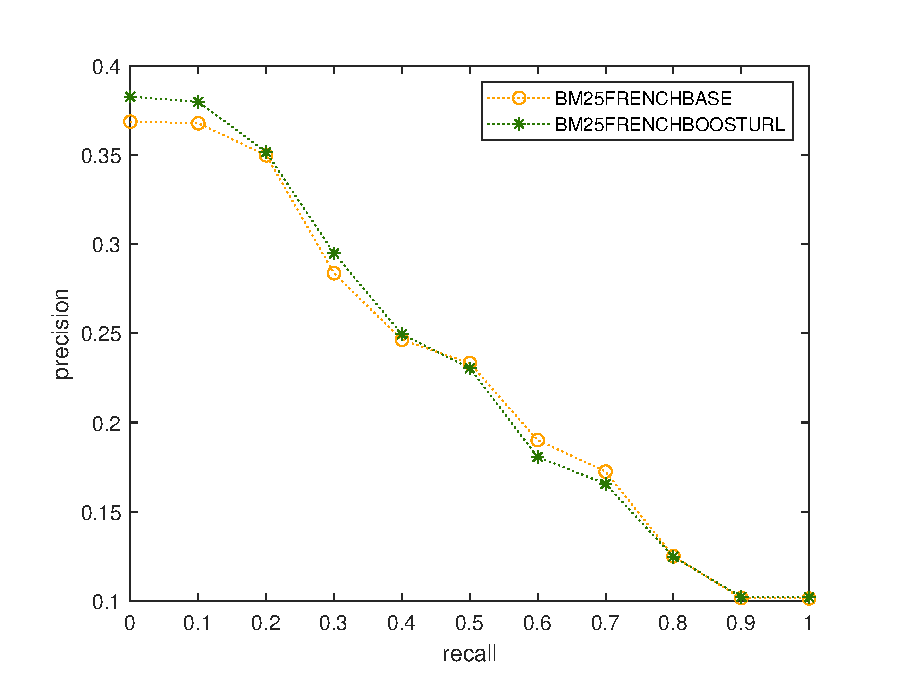
\includegraphics[scale=0.8]{figure/curve.eps}
    \caption{Interpolated precision-recall curve}
    \label{fig:prcurve}
\end{figure}



\subsection{Performance on Test Data}
\label{subsec:perfs}
Table~\ref{tab:sysperftest} reports the results computed for our CLEF-submitted systems over the LongEval test datasets. Each metric group represents a different indexing scenario, whether on same-time (of training data), short term evolution or long term evolution.
\begin{table}[tb]
  \caption{Test-time systems performance overview (nDCG)}
  \label{tab:sysperftest}
  \centering
  \begin{tabular}{|l|l|l|l|l|l|l|}
    \toprule
    \multirow{2}{*}{System name} & \multicolumn{2}{|c|}{Within Time} & \multicolumn{2}{|c|}{Short Term} & \multicolumn{2}{|c|}{Long Term}\\ 
    & nDCG & Recall@1000 & nDCG & Recall@1000 & nDCG & Recall@1000\\
    \midrule
    \textbf{BM25FRENCHBOOSTURL} & \textbf{0.3859} & \textbf{0.8708} & \textbf{0.3866} & \textbf{0.8323} & \textbf{0.3945} & \textbf{0.8556}\\
    BM25FRENCHBASE & 0.3843 & 0.8684 & 0.3924 & 0.8375 & 0.3916 & 0.8531\\
    BM25FRENCHRERANK100 & 0.3755 & 0.8644 & 0.3756 & 0.8365 & 0.3758 & 0.8531\\
    BM25FRENCHSPAM & 0.3605 & 0.7874 & 0.368 & 0.7686 & 0.3643 & 0.7773\\
    BM25TRANSLATEDQUERIES & 0.3072 & 0.7317 & 0.3051 & 0.7225 & 0.3189 & 0.7482\\
  \bottomrule
\end{tabular}
\end{table}
\par The results in Table~\ref{tab:sysperftest} highlight how the time-wise evolution of corpora (and queries) did not affect the system's effectiveness in any relevant way. This can be traced back to two main reasons:
\begin{itemize}
    \item The systems rely on language-specific components only for a minimal part. Moreover, such components are not largely affected by language change over time: unless way longer timespans are observed, stopwords are unlikely to change and filters working on syntax and morphology are expected to keep their behavior.
    \item At design time, during error analysis, changes were implemented targeting frequent problems that affected documents of various nature and content. Problems affecting specific categories of documents with specific content were not considered of primary interest as a means to avoid overfitting when given potentially different content to index.
\end{itemize}


\subsection{Hypothesis Testing \& Failure Analysis}
\label{subsec:hypotest}
To compare the submitted systems for each of the three case studies (withing time, short term and long term) we first plotted the box plots to have a visual representation of the systems, their mean and their variance. After that, we computed the two-way \ac{ANOVA} considering as hypothesis the null hypothesis  $H_0: \mu_x = \mu_y$ (where $x$ and $y$ represent two generic systems to be compared). The reason why we considered two-way \ac{ANOVA} and not one-way \ac{ANOVA} is that two-way \ac{ANOVA} considers both the topics and the systems effect while the one-way \ac{ANOVA} considers only the systems effect. The threshold that we used to consider the systems different was $\alpha=0.05$ (5\%). The results of the various \ac{ANOVA} tests have been reported in Table~\ref{tab:WTANOVA}, Table~\ref{tab:STANOVA} and Table~\ref{tab:LTANOVA}, where with SS we mean "Sum of Squares", with df we mean "degrees of freedom", with MS we mean "Mean Squares", with F we indicate the F-Test value and with prob>F we indicate the P-Value.
\par
Eventually, we computed the Tukey HSD Test to understand which of the systems were actually different (in Figure~\ref{fig:wthsd}, Figure~\ref{fig:sthsd} and Figure~\ref{fig:lthsd} the system highlighted in blue is the one considered for the comparison, the systems in red are the systems that are considered different, while the systems in grey are the systems that are considered similar). In all cases, the metric selected for the comparison has been the nDCG.

\subsubsection{Within Time}
\label{subsubsec:wt}
From the Box plots reported in Figure~\ref{fig:WTBP} we can see that the systems, in this case, appear to be quite similar.
\begin{figure}[tb]
    \centering
    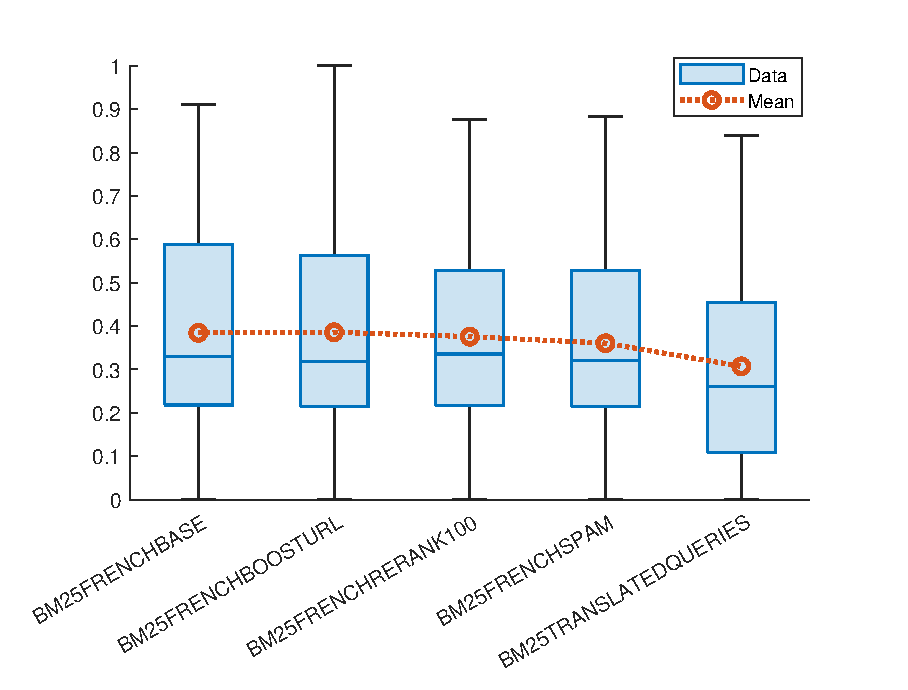
\includegraphics[scale=0.8]{figure/heldout/boxplot.eps}
    \caption{Box Plots Within Time}
    \label{fig:WTBP}
\end{figure}
This is not confirmed by the output of \ac{ANOVA} reported in Table~\ref{tab:WTANOVA} since the P-Value result to be lower than the considered threshold. Nonetheless, the results can be considered reliable since the system contribution is much higher than the error contribution.
\begin{table}[tb]
  \caption{Two-Way ANOVA Within Time (based on nDCG)}
  \label{tab:WTANOVA}
  \centering
  \begin{tabular}{|l|l|l|l|l|l|}
    \toprule
    Source & SS & df & MS & F & prob>F\\
    \midrule
    Columns (systems) & 0.4170 & 4 & 0.1042 & 8.2753 & 2.0570e-06\\
    Rows (topics) & 21.6586 & 97 & 0.2233 & 17.7255 & 1.1527e-97\\
    Error & 4.8876 & 388 & 0.0126 &  & \\
    Total & 26.9631 & 489 &  &  & \\
  \bottomrule
\end{tabular}
\end{table}
The ANOVA results highlight significant differences between the systems we have analyzed. This difference may be mainly due to the presence of an English-based system (\textit{BM25TRANSLATEDQUERIES}) along French-based ones.
\begin{figure}[p]
     \centering
     \begin{subfigure}[b]{0.49\textwidth}
         \centering
         \includegraphics[width=\textwidth]{figure/heldout/tukeyhsd-1.eps}
         \caption{BM25FRENCHBOOSTURL}
         \label{fig:wthsd1}
     \end{subfigure}
     \hfill
     \begin{subfigure}[b]{0.49\textwidth}
         \centering
         \includegraphics[width=\textwidth]{figure/heldout/tukeyhsd-2.eps}
         \caption{BM25FRENCHBASE}
         \label{fig:wthsd2}
     \end{subfigure}
     \hfill
     \begin{subfigure}[b]{0.49\textwidth}
         \centering
         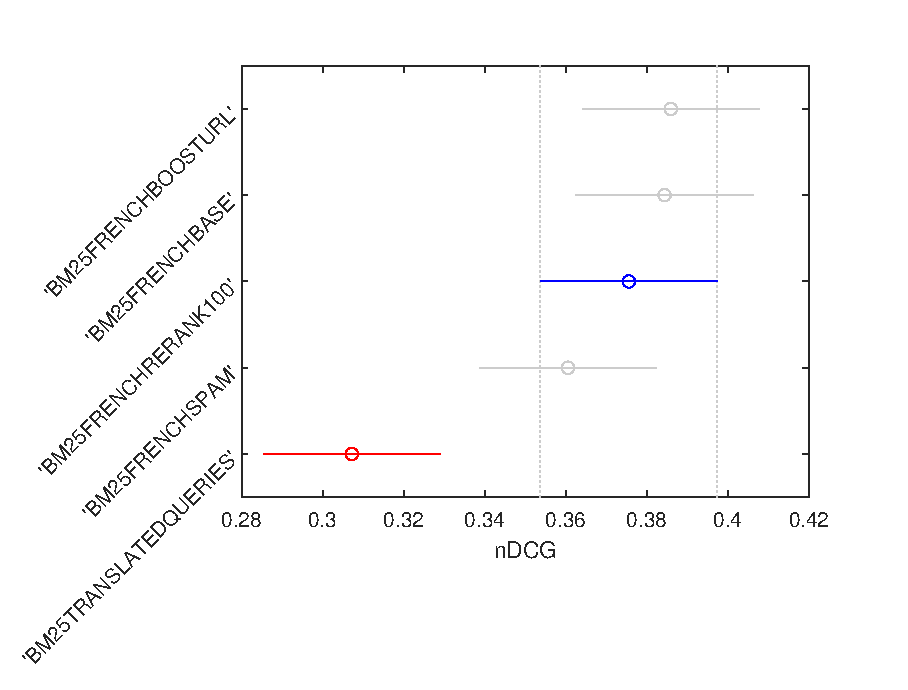
\includegraphics[width=\textwidth]{figure/heldout/tukeyhsd-3.eps}
         \caption{BM25FRENCHRERANK100}
         \label{fig:wthsd3}
     \end{subfigure}
     \begin{subfigure}[b]{0.49\textwidth}
         \centering
         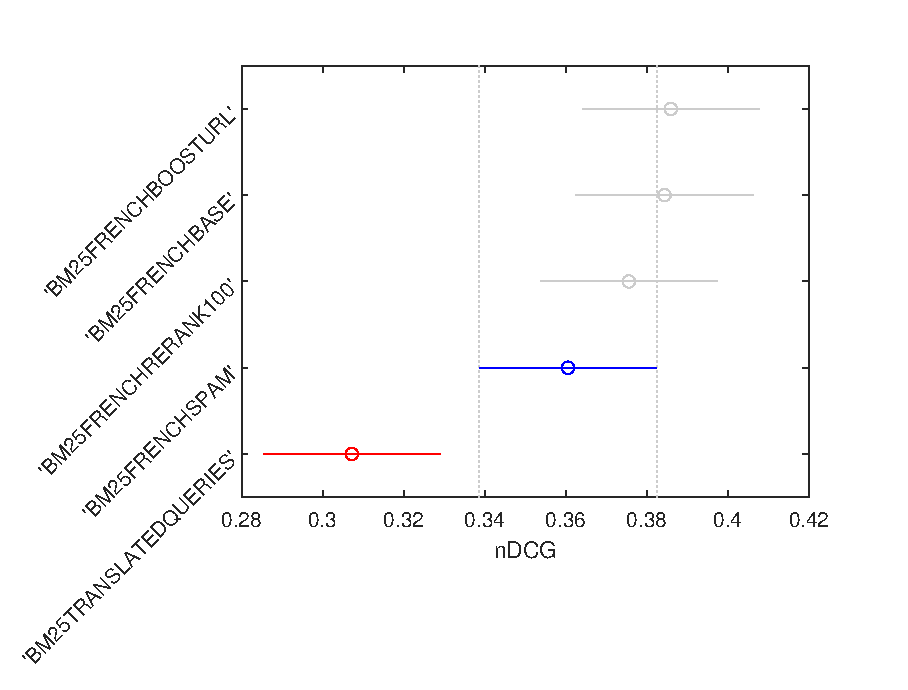
\includegraphics[width=\textwidth]{figure/heldout/tukeyhsd-4.eps}
         \caption{BM25FRENCHSPAM}
         \label{fig:wthsd4}
     \end{subfigure}
     \begin{subfigure}[b]{0.49\textwidth}
         \centering
         \includegraphics[width=\textwidth]{figure/heldout/tukeyhsd-5.eps}
         \caption{BM25TRANSLATEDQUERIES}
         \label{fig:wthsd5}
     \end{subfigure}
        \caption{Tukey HSD Test Within Time}
        \label{fig:wthsd}
\end{figure}
\par
Moreover, by looking at the Tukey HSD results (reported in Figure~\ref{fig:wthsd}) the only system that appears different from the others is the \textit{BM25TRANSLATEDQUERIES} system. This could be due to the fact that that system is the only one using the English corpus and the performance results to be quite different from the others.
\par
We can conclude that the systems are quite similar but the \textit{BM25TRANSLATEDQUERIES} system turns out to be the only one showing relevant differences.


\subsubsection{Short Term}
\label{subsubsec:st}
By looking at the box plot reported in Figure~\ref{fig:STBP} we see that the systems have pretty much the same performance, only \textit{BM25TRANSLATEDQUERIES} differs a bit from the others.
\begin{figure}[tb]
    \centering
    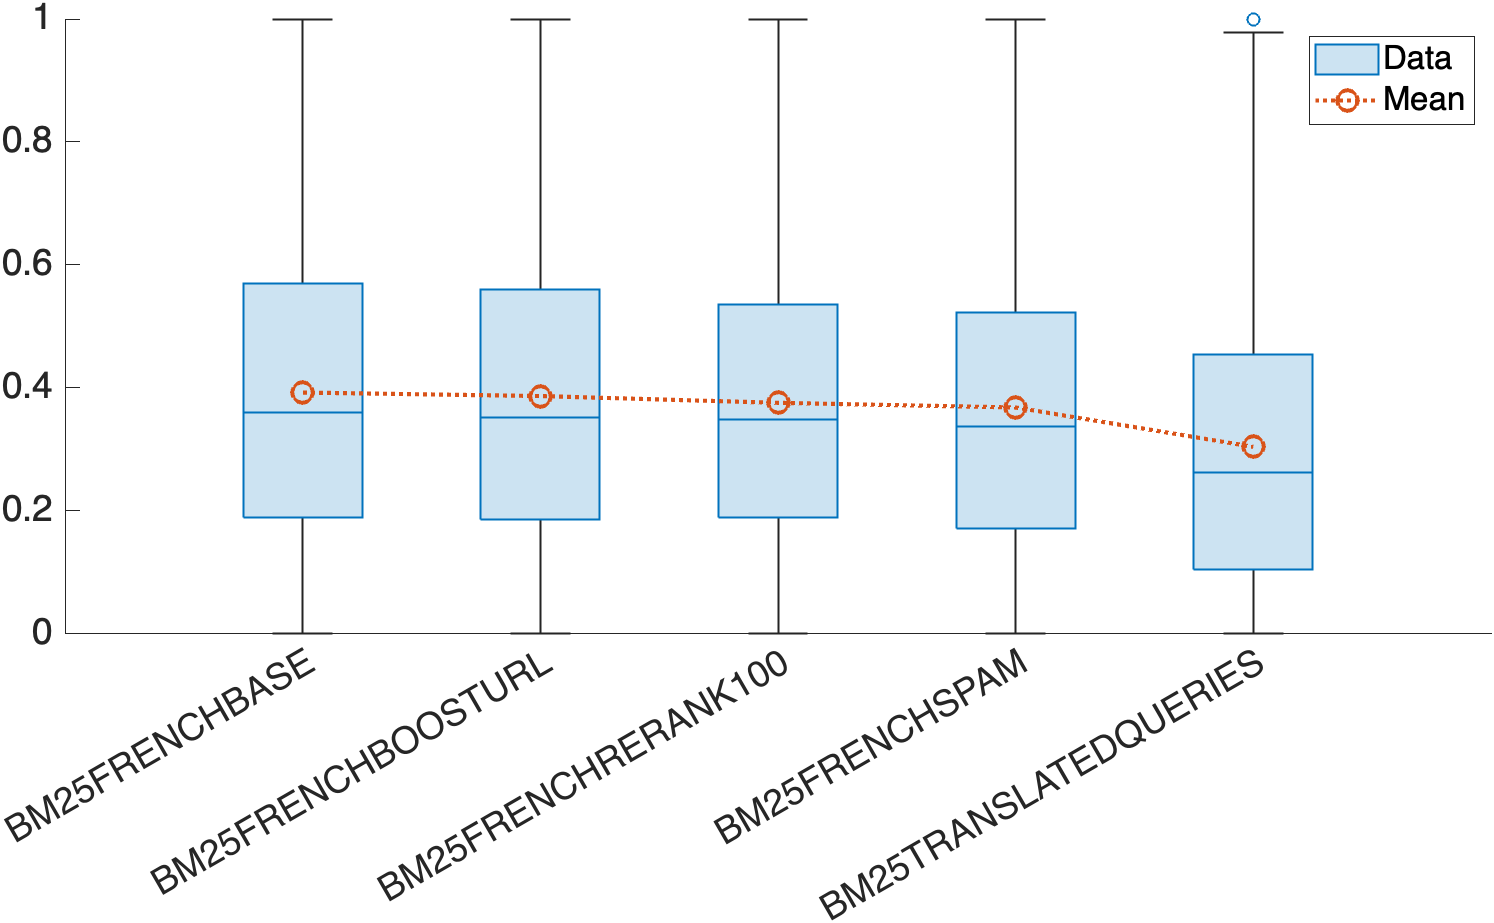
\includegraphics[scale=0.5]{figure/shortterm/boxplot.png}
    \caption{Box Plots Short Term}
    \label{fig:STBP}
\end{figure}
Furthermore we can see that the extension of the whiskers in almost all the systems goes from 0 to 1, this is due to the fact that those systems performs very well for some queries (and reach the maximum value of nDCG) but very poorly for some other queries. A deeper analysis of the results revealed that the queries performing well were very specific while the ones performing badly were either or generic queries or containing terms that can be considered spam (see Section~\ref{subsubsec:spam} for more details).
\par
The two-way \ac{ANOVA} (whose results are reported in Table~\ref{tab:STANOVA}) does reveal relevant differences among the systems since the P-Value result to be lower than the considered threshold. Furthermore, the results of \ac{ANOVA} can be considered reliable since the system contribution is much higher than the error contribution.
\begin{table}[tb]
  \caption{Two-Way ANOVA Short Time (based on nDCG)}
  \label{tab:STANOVA}
  \centering
  \begin{tabular}{|l|l|l|l|l|l|}
    \toprule
    Source & SS & df & MS & F & prob>F\\
    \midrule
    Columns (systems) & 4.4582 & 4 & 1.1145 & 87.3582 & 7.1783e-71\\
    Rows (topics) & 231.3659 & 881 & 0.2626 & 20.5839 & 0\\
    Error & 44.9605 & 3524 & 0.0128 &  & \\
    Total & 280.7846 & 4409 &  &  & \\
  \bottomrule
\end{tabular}
\end{table}
\par
By looking at the Tukey HSD results (reported in Figure~\ref{fig:sthsd}) we noticed that there is a clear difference between \textit{BM25TRANSLATEDQUERIES} and the other systems, this is due to the fact that this system is based on the English collection. Taken the best system's test (\textit{BM25FRENCHBASE}'s), we see that the \textit{BM25FRENCHBASE} system is significantly different from all systems other than the \textit{BM25FRENCHBOOSTURL} system, this happens because they are basically the same except that the \textit{BM25FRENCHBOOSTURL} system uses an additional field: the URL.
\begin{figure}[tb]
     \centering
     \begin{subfigure}[b]{0.49\textwidth}
         \centering
         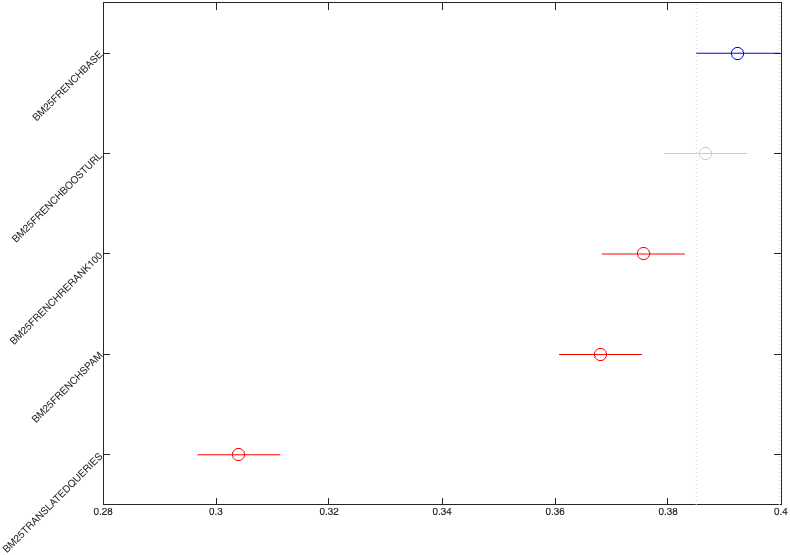
\includegraphics[width=\textwidth]{figure/shortterm/tukeyhsd-1.png}
         \caption{BM25FRENCHBASE}
         \label{fig:sthsd1}
     \end{subfigure}
     \hfill
     \begin{subfigure}[b]{0.49\textwidth}
         \centering
         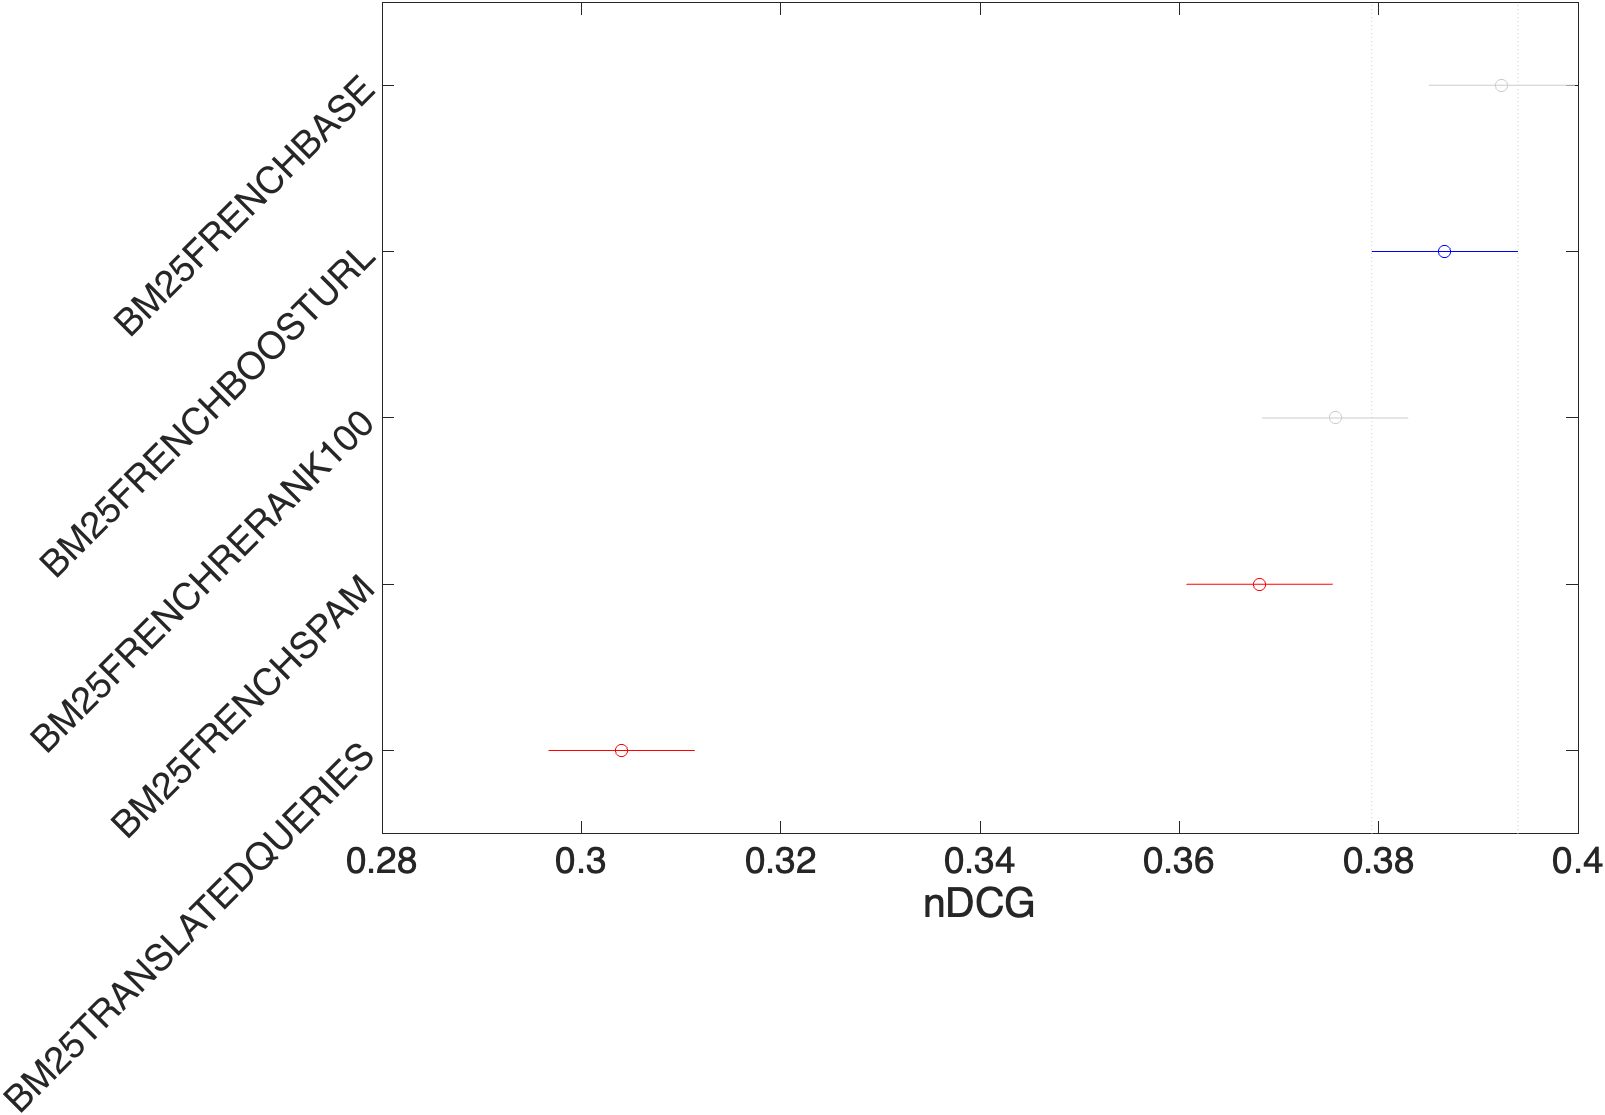
\includegraphics[width=\textwidth]{figure/shortterm/tukeyhsd-2.png}
         \caption{BM25FRENCHBOOSTURL}
         \label{fig:sthsd2}
     \end{subfigure}
     \hfill
     \begin{subfigure}[b]{0.49\textwidth}
         \centering
         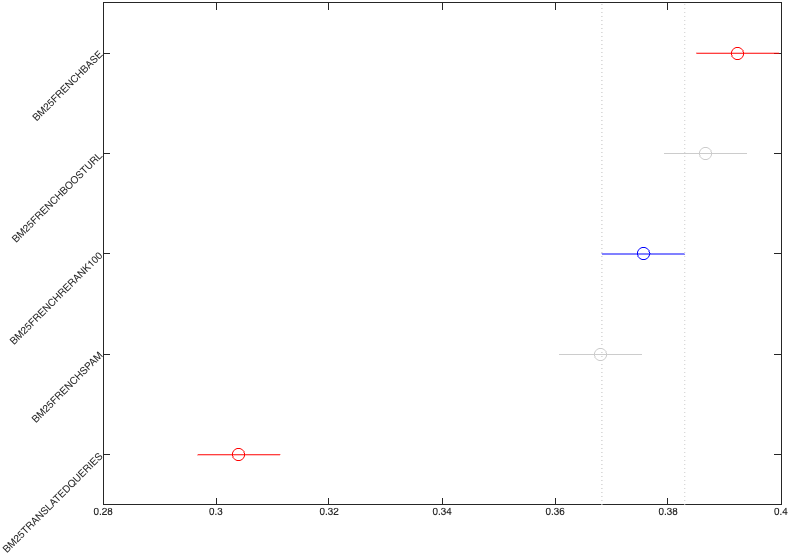
\includegraphics[width=\textwidth]{figure/shortterm/tukeyhsd-3.png}
         \caption{BM25FRENCHRERANK100}
         \label{fig:sthsd3}
     \end{subfigure}
     \begin{subfigure}[b]{0.49\textwidth}
         \centering
         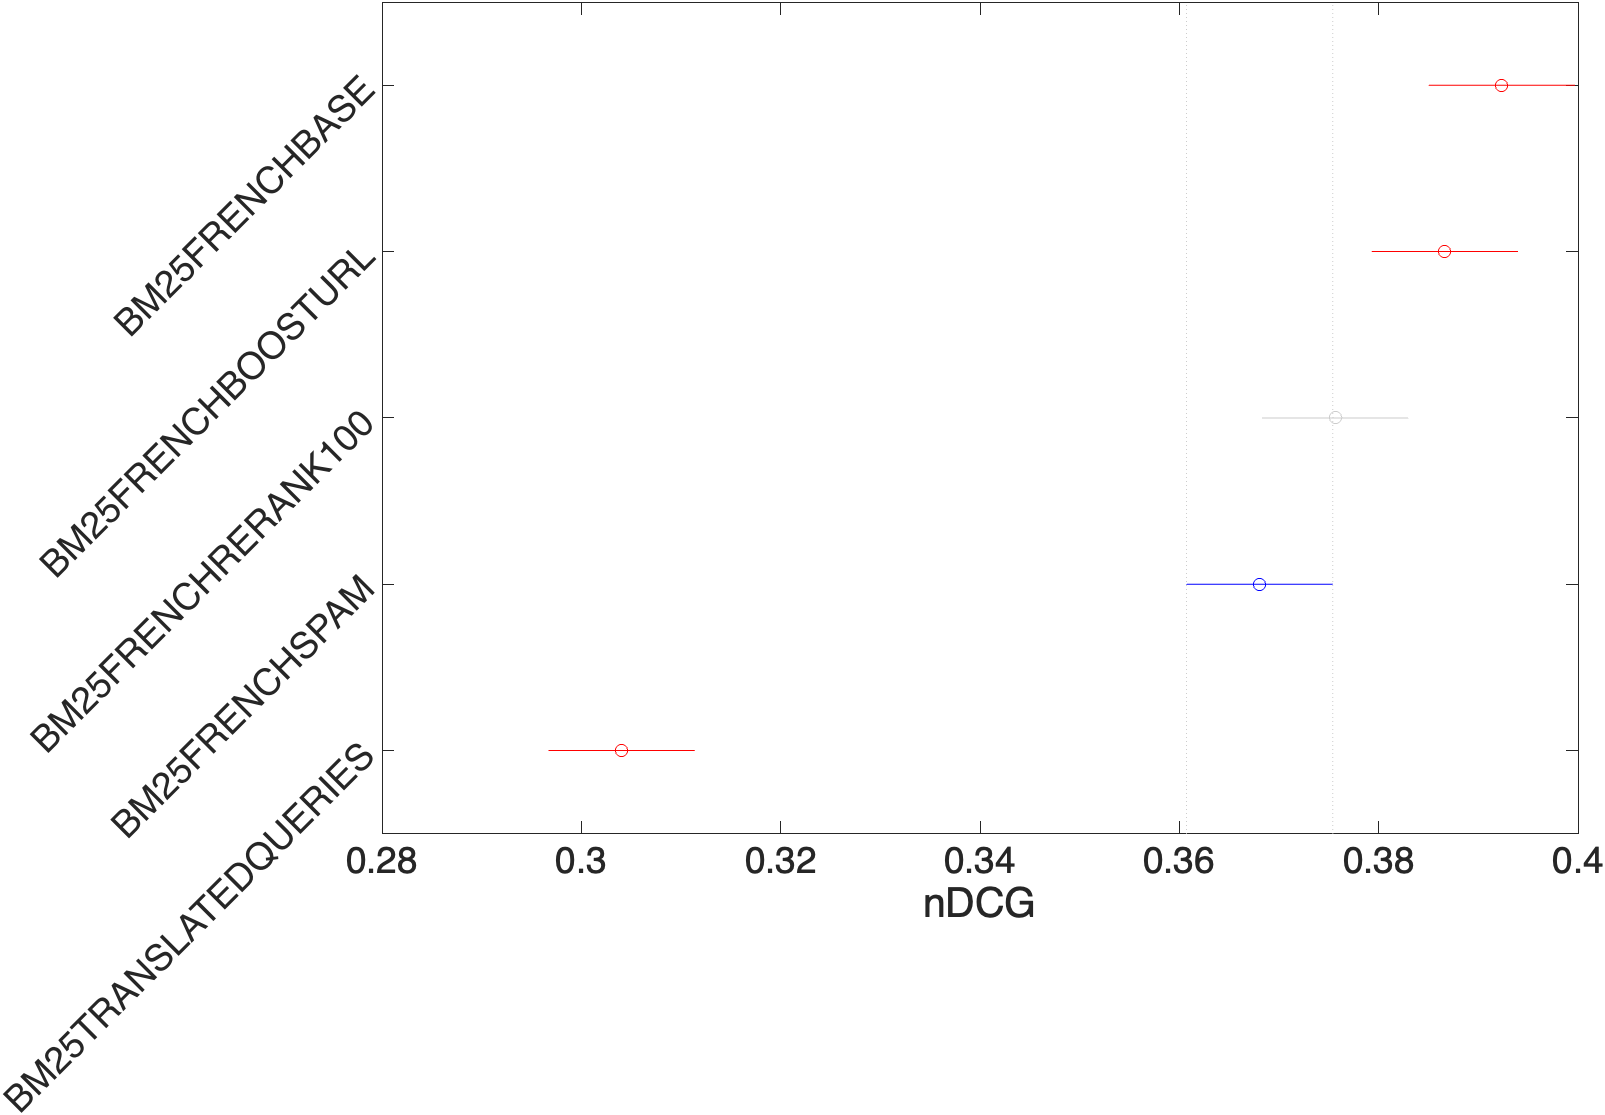
\includegraphics[width=\textwidth]{figure/shortterm/tukeyhsd-4.png}
         \caption{BM25FRENCHSPAM}
         \label{fig:sthsd4}
     \end{subfigure}
     \begin{subfigure}[b]{0.49\textwidth}
         \centering
         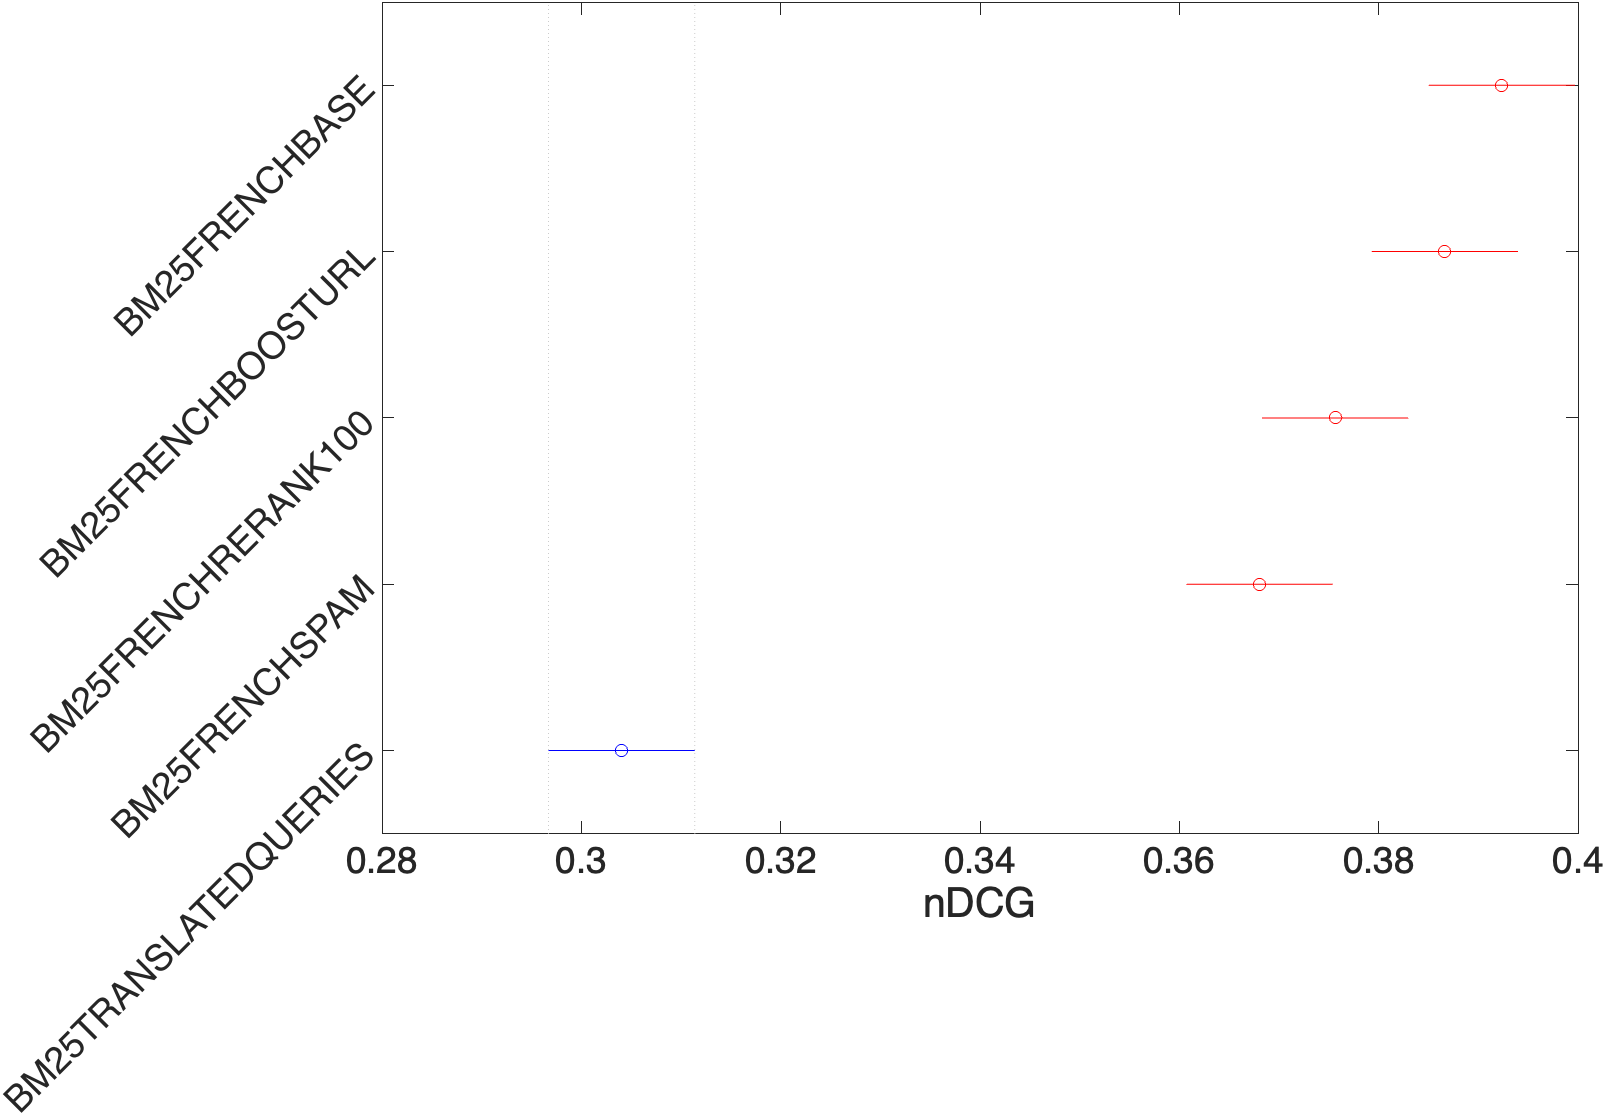
\includegraphics[width=\textwidth]{figure/shortterm/tukeyhsd-5.png}
         \caption{BM25TRANSLATEDQUERIES}
         \label{fig:sthsd5}
     \end{subfigure}
        \caption{Tukey HSD Test Short Term}
        \label{fig:sthsd}
\end{figure}


\subsubsection{Long Term}
\label{subsubsec:lt}
From the Box plots reported in Figure~\ref{fig:LTBP} we can see that the systems, even in this case, appear to be quite similar.
\begin{figure}[tb]
    \centering
    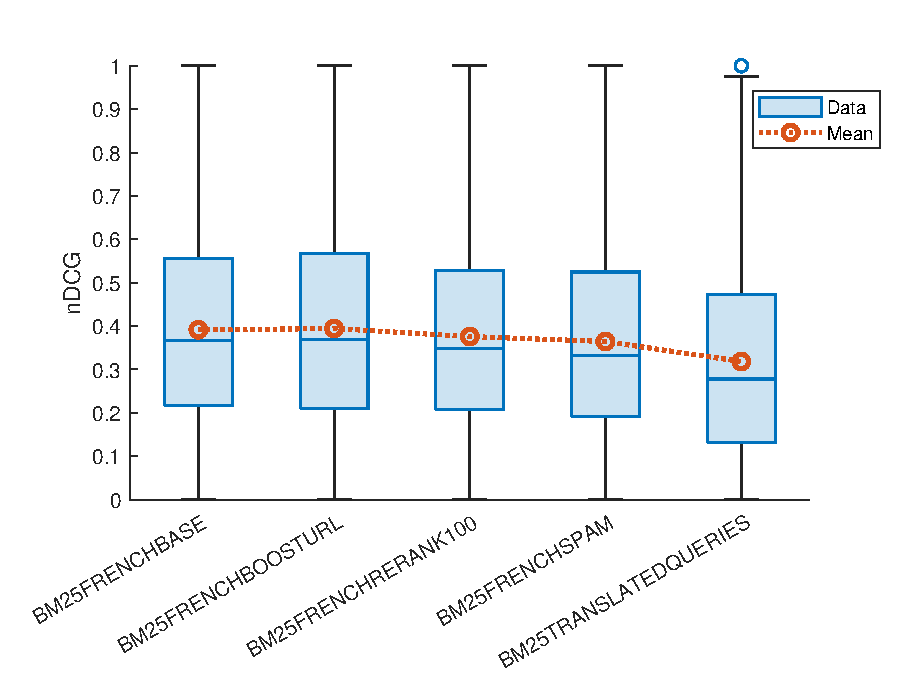
\includegraphics[scale=0.8]{figure/longterm/boxplot.eps}
    \caption{Box Plots Long Term}
    \label{fig:LTBP}
\end{figure}
Furthermore we can see that the extension of the whiskers in almost all the systems goes from 0 to 1, this is due to the fact that those systems performs very well for some queries (and reach the maximum value of nDCG) but very poorly for some other queries. A deeper analysis of the results revealed that the queries performing well were very specific while the ones performing badly were either or generic queries or containing terms that can be considered spam (see Section~\ref{subsubsec:spam} for more details).
\par
The two-way \ac{ANOVA} (whose results are reported in Table~\ref{tab:LTANOVA}) does reveal relevant differences among the systems since the P-Value result to be lower than the considered threshold. Furthermore, the results of \ac{ANOVA} can be considered reliable since the system contribution is much higher than the error contribution.
\begin{table}[tb]
  \caption{Two-Way ANOVA Long Time (based on nDCG)}
  \label{tab:LTANOVA}
  \centering
  \begin{tabular}{|l|l|l|l|l|l|}
    \toprule
    Source & SS & df & MS & F & prob>F\\
    \midrule
    Columns (systems) & 3.5172 & 4 & 0.8793 & 79.2206 & 1.4254e-64\\
    Rows (topics) & 218.3013 & 992 & 0.2368 & 21.3319 & 0\\
    Error & 40.9342 & 3688 & 0.0111 &  & \\
    Total & 262.7527 & 4614 &  &  & \\
  \bottomrule
\end{tabular}
\end{table}
\par
By looking at the Tukey HSD results (reported in Figure~\ref{fig:lthsd}) we noticed that the two best performing systems (\textit{BM25FRENCHBOOSTURL} and \textit{BM25FRENCHBASE}) happen to be quite similar between each other but different from the other systems; this happens because the \textit{BM25FRENCHBOOSTURL} system is actually the same as the \textit{BM25FRENCHBASE} system except that is uses one additional field: the URL. Furthermore, also the \textit{BM25FRENCHRERANK100} system and the \textit{BM25FRENCHSPAM} turn out to be similar while the \textit{BM25TRANSLATEDQUERIES} system still looks different and (as in the previous case studies) this is due to the fact that this last system is based on the English collection.  
\begin{figure}[p]
     \centering
     \begin{subfigure}[b]{0.49\textwidth}
         \centering
         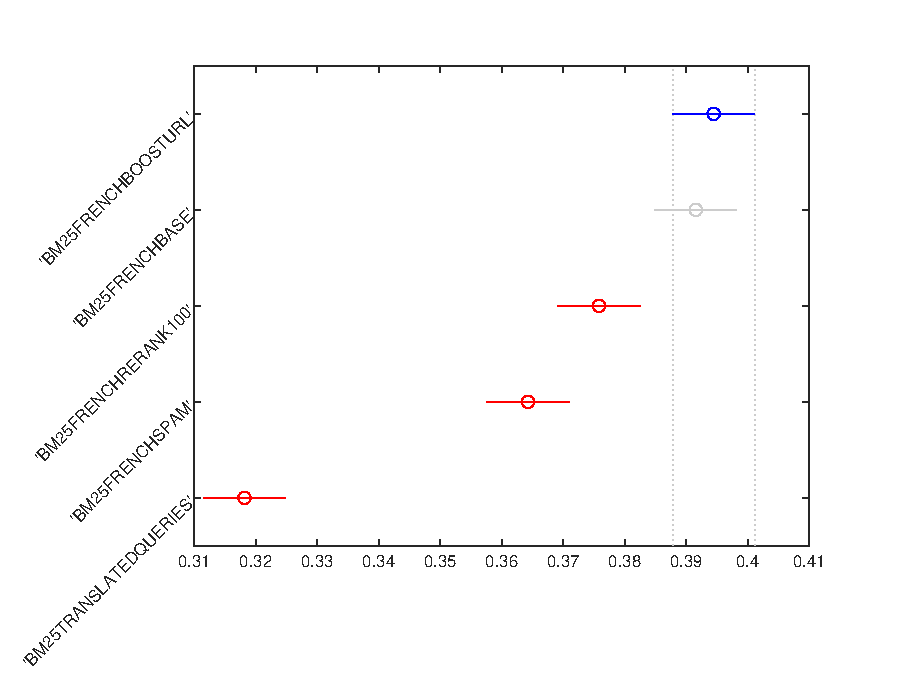
\includegraphics[width=\textwidth]{figure/longterm/tukeyhsd-1.eps}
         \caption{BM25FRENCHBOOSTURL}
         \label{fig:lthsd1}
     \end{subfigure}
     \hfill
     \begin{subfigure}[b]{0.49\textwidth}
         \centering
         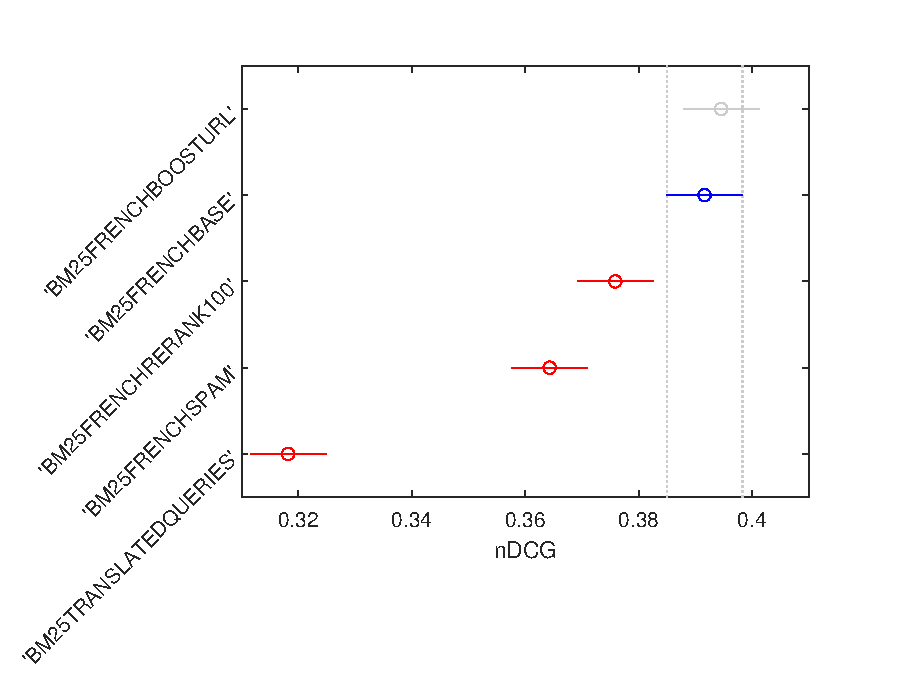
\includegraphics[width=\textwidth]{figure/longterm/tukeyhsd-2.eps}
         \caption{BM25FRENCHBASE}
         \label{fig:lthsd2}
     \end{subfigure}
     \hfill
     \begin{subfigure}[b]{0.49\textwidth}
         \centering
         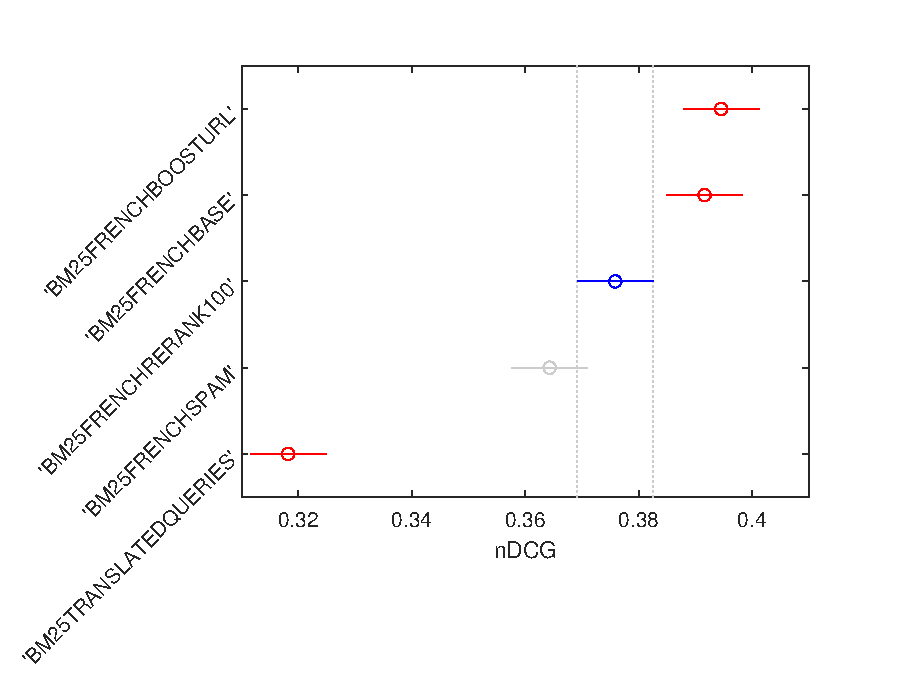
\includegraphics[width=\textwidth]{figure/longterm/tukeyhsd-3.eps}
         \caption{BM25FRENCHRERANK100}
         \label{fig:lthsd3}
     \end{subfigure}
     \begin{subfigure}[b]{0.49\textwidth}
         \centering
         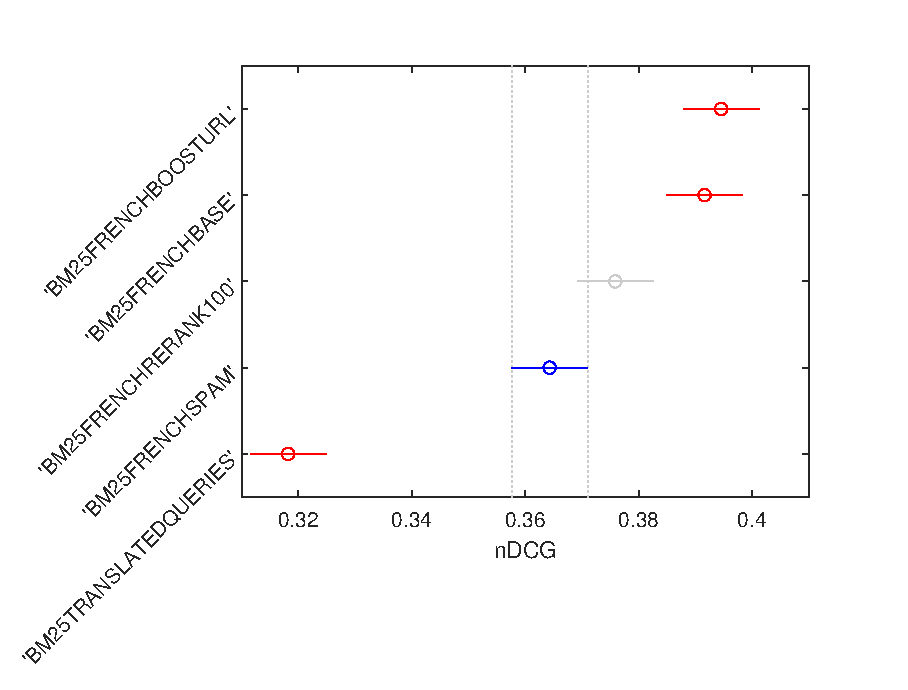
\includegraphics[width=\textwidth]{figure/longterm/tukeyhsd-4.eps}
         \caption{BM25FRENCHSPAM}
         \label{fig:lthsd4}
     \end{subfigure}
     \begin{subfigure}[b]{0.49\textwidth}
         \centering
         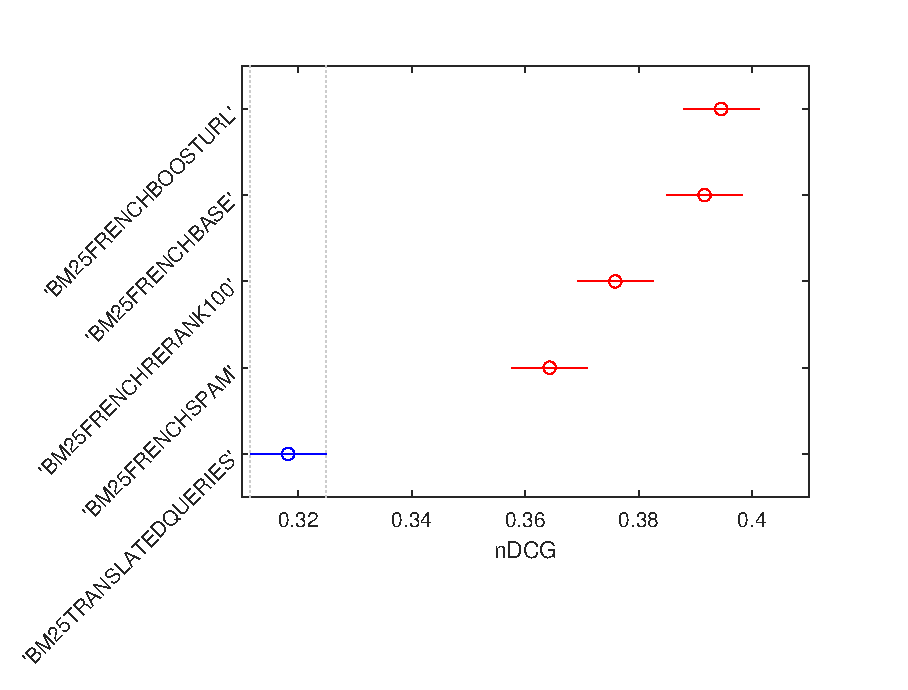
\includegraphics[width=\textwidth]{figure/longterm/tukeyhsd-5.eps}
         \caption{BM25TRANSLATEDQUERIES}
         \label{fig:lthsd5}
     \end{subfigure}
        \caption{Tukey HSD Test Long Term}
        \label{fig:lthsd}
\end{figure}

\section{Conclusions and Future Work}
\label{sec:conclusion}

Provide a summary of what are the main achievements and findings. 

Discuss future work, e.g. what you may try next and/or how your approach could be further developed.


\section{Misc [TO BE REMOVED]}

\subsection{Tex Files}

Put your \LaTeX files into the \texttt{section} folder as shown in the examples above.

\subsection{Figures}

Put your figures into the \texttt{figure} folder and put the caption under the figure. Example of reference to Figure~\ref{fig:sample-figure}.

\begin{figure}
  \centering
  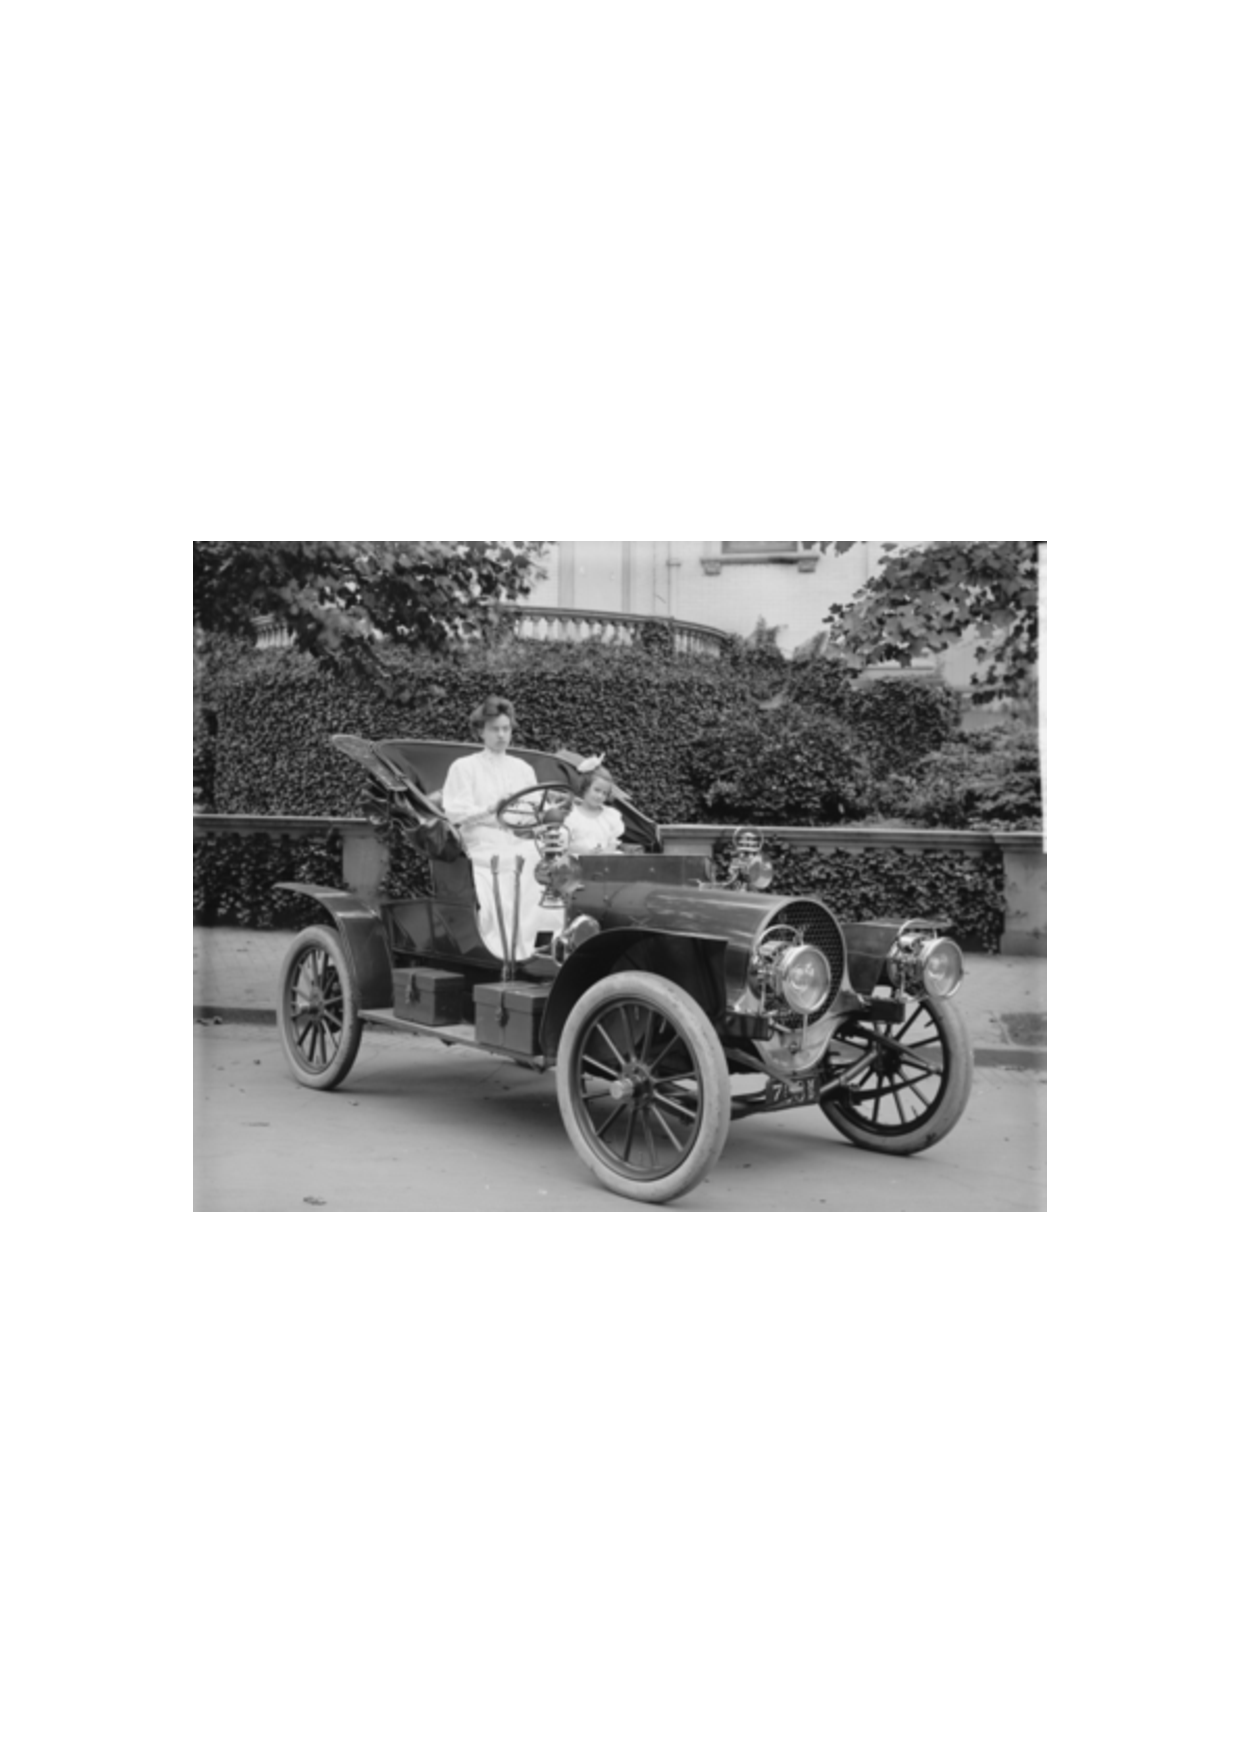
\includegraphics[width=0.8\linewidth]{figure/sample.pdf}
  \caption{1907 Franklin Model D roadster. Photograph by Harris \& Ewing, Inc. [Public domain], via Wikimedia Commons. (\url{https://goo.gl/VLCRBB}).}
  \label{fig:sample-figure}
\end{figure}

\subsection{Tables}

Put the caption above the table. Example of reference to Table~\ref{tab:sample-table}.

\begin{table}
  \caption{Frequency of Special Characters}
  \label{tab:sample-table}
  \centering
  \begin{tabular}{|c|c|l|}
    \toprule
    Non-English or Math&Frequency&Comments\\
    \midrule
    \O & 1 in 1,000& For Swedish names\\
    $\pi$ & 1 in 5& Common in math\\
    \$ & 4 in 5 & Used in business\\
    $\Psi^2_1$ & 1 in 40,000& Unexplained usage\\
  \bottomrule
\end{tabular}
\end{table}

See the \texttt{booktab} packaged documentation for further options.

\subsection{Bibliography}

Example of citations:
\begin{itemize}
	\item name: \citet{Salton1968}
	\item parenthesis: \citep{Salton1968}
\end{itemize}

An initial list of references is provided in the files \texttt{bibliography.bib} and \texttt{proceedings.bib} that you can expand.

See the \texttt{natbib} packaged documentation for further options.

\subsection{Acronyms}

Use the 

\begin{verbatim}
 \ac{acronym}
 \end{verbatim}

command to insert acronyms, eg. \ac{AP}. The command will expand the acronym the first time it is used.

An initial list of acronyms is provided in the file \texttt{acronyms.tex} that you can expand.

See the \texttt{acronym} packaged documentation for further options.


%% Define the bibliography file to be used
\bibliography{bibliography,proceedings}

\acrodef{3G}[3G]{Third Generation Mobile System}
\acrodef{5S}[5S]{Streams, Structures, Spaces, Scenarios, Societies}
\acrodef{AA}[AA]{Active Agreements}
\acrodef{AAAI}[AAAI]{Association for the Advancement of Artificial Intelligence}
\acrodef{AAL}[AAL]{Annotation Abstraction Layer}
\acrodef{AAM}[AAM]{Automatic Annotation Manager}
\acrodef{AAP}[AAP]{Average Average Precision}
\acrodef{ACLIA}[ACLIA]{Advanced Cross-Lingual Information Access}
\acrodef{ACM}[ACM]{Association for Computing Machinery}
\acrodef{AD}[AD]{Active Disagreements}
\acrodef{ADSL}[ADSL]{Asymmetric Digital Subscriber Line}
\acrodef{ADUI}[ADUI]{ADministrator User Interface}
\acrodef{AIP}[AIP]{Archival Information Package}
\acrodef{AJAX}[AJAX]{Asynchronous JavaScript Technology and \acs{XML}}
\acrodef{ALU}[ALU]{Aritmetic-Logic Unit}
\acrodef{AMUSID}[AMUSID]{Adaptive MUSeological IDentity-service}
\acrodef{ANOVA}[ANOVA]{ANalysis Of VAriance}
\acrodef{ANSI}[ANSI]{American National Standards Institute}
\acrodef{AP}[AP]{Average Precision}
\acrodef{APC}[APC]{AP Correlation}
\acrodef{API}[API]{Application Program Interface}
\acrodef{AR}[AR]{Address Register}
\acrodef{AS}[AS]{Annotation Service}
\acrodef{ASAP}[ASAP]{Adaptable Software Architecture Performance}
\acrodef{ASI}[ASI]{Annotation Service Integrator}
\acrodef{ASL}[ASL]{Achieved Significance Level}
\acrodef{ASM}[ASM]{Annotation Storing Manager}
\acrodef{ASR}[ASR]{Automatic Speech Recognition}
\acrodef{ASUI}[ASUI]{ASsessor User Interface}
\acrodef{ATIM}[ATIM]{Annotation Textual Indexing Manager}
\acrodef{AUC}[AUC]{Area Under the ROC Curve}
\acrodef{AUI}[AUI]{Administrative User Interface}
\acrodef{AWARE}[AWARE]{Assessor-driven Weighted Averages for Retrieval Evaluation}
\acrodef{BANKS-I}[BANKS-I]{Browsing ANd Keyword Searching I}
\acrodef{BANKS-II}[BANKS-II]{Browsing ANd Keyword Searching II}
\acrodef{BH}[BH]{Benjamini-Hochberg}
\acrodef{bpref}[bpref]{Binary Preference}
\acrodef{BNF}[BNF]{Backus and Naur Form}
\acrodef{BPM}[BPM]{Bejeweled Player Model}
\acrodef{BRICKS}[BRICKS]{Building Resources for Integrated Cultural Knowledge Services}
\acrodef{CAN}[CAN]{Content Addressable Netword}
\acrodef{CAS}[CAS]{Content-And-Structure}
\acrodef{CBSD}[CBSD]{Component-Based Software Developlement}
\acrodef{CBSE}[CBSE]{Component-Based Software Engineering}
\acrodef{CB-SPE}[CB-SPE]{Component-Based \acs{SPE}}
\acrodef{CD}[CD]{Collaboration Diagram}
\acrodef{CD}[CD]{Compact Disk}
\acrodef{CDF}[CDF]{Cumulative Density Function}
\acrodef{CENL}[CENL]{Conference of European National Librarians}
\acrodef{CIDOC CRM}[CIDOC CRM]{CIDOC Conceptual Reference Model}
\acrodef{CIR}[CIR]{Current Instruction Register}
\acrodef{CIRCO}[CIRCO]{Coordinated Information Retrieval Components Orchestration}
\acrodef{CG}[CG]{Cumulated Gain}
\acrodef{CL}[CL]{Curriculum Learning}
\acrodef{CL-ESA}[CL-ESA]{Cross-Lingual Explicit Semantic Analysis}
\acrodef{CLAIRE}[CLAIRE]{Combinatorial visuaL Analytics system for Information Retrieval Evaluation}
\acrodef{CLEF1}[CLEF]{Cross-Language Evaluation Forum}
\acrodef{CLEF}[CLEF]{Conference and Labs of the Evaluation Forum}
\acrodef{CLIR}[CLIR]{Cross Language Information Retrieval}
\acrodef{CM}[CM]{Continuation Methods}
\acrodef{CMS}[CMS]{Content Management System}
\acrodef{CMT}[CMT]{Campaign Management Tool}
\acrodef{CNR}[CNR]{Italian National Council of Research}
\acrodef{CO}[CO]{Content-Only}
\acrodef{COD}[COD]{Code On Demand}
\acrodef{CODATA}[CODATA]{Committee on Data for Science and Technology}
\acrodef{COLLATE}[COLLATE]{Collaboratory for Annotation Indexing and Retrieval of Digitized Historical Archive Material}
\acrodef{CP}[CP]{Characteristic Pattern}
\acrodef{CPE}[CPE]{Control Processor Element}
\acrodef{CPU}[CPU]{Central Processing Unit}
\acrodef{CQL}[CQL]{Contextual Query Language}
\acrodef{CRP}[CRP]{Cumulated Relative Position}
\acrodef{CRUD}[CRUD]{Create--Read--Update--Delete}
\acrodef{CS}[CS]{Characteristic Structure}
\acrodef{CSM}[CSM]{Campaign Storing Manager}
\acrodef{CSS}[CSS]{Cascading Style Sheets}
\acrodef{CTR}[CTR]{Click-Through Rate}
\acrodef{CU}[CU]{Control Unit}
\acrodef{CUI}[CUI]{Client User Interface}
\acrodef{CV}[CV]{Cross-Validation}
\acrodef{DAFFODIL}[DAFFODIL]{Distributed Agents for User-Friendly Access of Digital Libraries}
\acrodef{DAO}[DAO]{Data Access Object}
\acrodef{DARE}[DARE]{Drawing Adequate REpresentations}
\acrodef{DARPA}[DARPA]{Defense Advanced Research Projects Agency}
\acrodef{DAS}[DAS]{Distributed Annotation System}
\acrodef{DB}[DB]{DataBase}
\acrodef{DBMS}[DBMS]{DataBase Management System}
\acrodef{DC}[DC]{Dublin Core}
\acrodef{DCG}[DCG]{Discounted Cumulated Gain}
\acrodef{DCMI}[DCMI]{Dublin Core Metadata Initiative}
\acrodef{DCV}[DCV]{Document Cut--off Value}
\acrodef{DD}[DD]{Deployment Diagram}
\acrodef{DDC}[DDC]{Dewey Decimal Classification}
\acrodef{DDS}[DDS]{Direct Data Structure}
\acrodef{DF}[DF]{Degrees of Freedom}
\acrodef{DFI}[DFI]{Divergence From Independence}
\acrodef{DFR}[DFR]{Divergence From Randomness}
\acrodef{DHT}[DHT]{Distributed Hash Table}
\acrodef{DI}[DI]{Digital Image}
\acrodef{DIKW}[DIKW]{Data, Information, Knowledge, Wisdom}
\acrodef{DIL}[DIL]{\acs{DIRECT} Integration Layer}
\acrodef{DiLAS}[DiLAS]{Digital Library Annotation Service}
\acrodef{DIRECT}[DIRECT]{Distributed Information Retrieval Evaluation Campaign Tool}
\acrodef{DKMS}[DKMS]{Data and Knowledge Management System}
\acrodef{DL}[DL]{Digital Library}
\acrodefplural{DL}[DL]{Digital Libraries}
\acrodef{DLMS}[DLMS]{Digital Library Management System}
\acrodef{DLOG}[DL]{Description Logics}
\acrodef{DLS}[DLS]{Digital Library System}
\acrodef{DLSS}[DLSS]{Digital Library Service System}
\acrodef{DM}[DM]{Data Mining}
\acrodef{DO}[DO]{Digital Object}
\acrodef{DOI}[DOI]{Digital Object Identifier}
\acrodef{DOM}[DOM]{Document Object Model}
\acrodef{DoMDL}[DoMDL]{Document Model for Digital Libraries}
\acrodef{DP}[DP]{Discriminative Power}
\acrodef{DPBF}[DPBF]{Dynamic Programming Best-First}
\acrodef{DR}[DR]{Data Register}
\acrodef{DRIVER}[DRIVER]{Digital Repository Infrastructure Vision for European Research}
\acrodef{DTD}[DTD]{Document Type Definition}
\acrodef{DVD}[DVD]{Digital Versatile Disk}
\acrodef{EAC-CPF}[EAC-CPF]{Encoded Archival Context for Corporate Bodies, Persons, and Families}
\acrodef{EAD}[EAD]{Encoded Archival Description}
\acrodef{EAN}[EAN]{International Article Number}
\acrodef{EBU}[EBU]{Expected Browsing Utility}
\acrodef{ECD}[ECD]{Enhanced Contenty Delivery}
\acrodef{ECDL}[ECDL]{European Conference on Research and Advanced Technology for Digital Libraries}
\acrodef{EDM}[EDM]{Europeana Data Model}
\acrodef{EG}[EG]{Execution Graph}
\acrodef{ELDA}[ELDA]{Evaluation and Language resources Distribution Agency}
\acrodef{ELRA}[ELRA]{European Language Resources Association}
\acrodef{EM}[EM]{Expectation Maximization}
\acrodef{EMMA}[EMMA]{Extensible MultiModal Annotation}
\acrodef{EPROM}[EPROM]{Erasable Programmable \acs{ROM}}
\acrodef{EQNM}[EQNM]{Extended Queueing Network Model}
\acrodef{ER}[ER]{Entity--Relationship}
\acrodef{ERR}[ERR]{Expected Reciprocal Rank}
\acrodef{ERS}[ERS]{Empirical Relational System}
\acrodef{ESA}[ESA]{Explicit Semantic Analysis}
\acrodef{ESL}[ESL]{Expected Search Length}
\acrodef{ETL}[ETL]{Extract-Transform-Load}
\acrodef{FAST}[FAST]{Flexible Annotation Service Tool}
\acrodef{FDR}[FDR]{False Discovery Rate}
\acrodef{FIFO}[FIFO]{First-In / First-Out}
\acrodef{FIRE}[FIRE]{Forum for Information Retrieval Evaluation}
\acrodef{FN}[FN]{False Negative}
\acrodef{FNR}[FNR]{False Negative Rate}
\acrodef{FOAF}[FOAF]{Friend of a Friend}
\acrodef{FORESEE}[FORESEE]{FOod REcommentation sErvER}
\acrodef{FP}[FP]{False Positive}
\acrodef{FPR}[FPR]{False Positive Rate}
\acrodef{FWER}[FWER]{Family-wise Error Rate}
\acrodef{GIF}[GIF]{Graphics Interchange Format}
\acrodef{GIR}[GIR]{Geografic Information Retrieval}
\acrodef{GAP}[GAP]{Graded Average Precision}
\acrodef{GLM}[GLM]{General Linear Model}
\acrodef{GLMM}[GLMM]{General Linear Mixed Model}
\acrodef{GMAP}[GMAP]{Geometric Mean Average Precision}
\acrodef{GoP}[GoP]{Grid of Points}
\acrodef{GPRS}[GPRS]{General Packet Radio Service}
\acrodef{gP}[gP]{Generalized Precision}
\acrodef{gR}[gR]{Generalized Recall}
\acrodef{gRBP}[gRBP]{Graded Rank-Biased Precision}
\acrodef{GT}[GT]{Generalizability Theory}
\acrodef{GTIN}[GTIN]{Global Trade Item Number}
\acrodef{GUI}[GUI]{Graphical User Interface}
\acrodef{GW}[GW]{Gateway}
\acrodef{HCI}[HCI]{Human Computer Interaction}
\acrodef{HDS}[HDS]{Hybrid Data Structure}
\acrodef{HIR}[HIR]{Hypertext Information Retrieval}
\acrodef{HIT}[HIT]{Human Intelligent Task}
\acrodef{HITS}[HITS]{Hyperlink-Induced Topic Search}
\acrodef{HMM}[HMM]{Hidden Markov Model}
\acrodef{HTML}[HTML]{HyperText Markup Language}
\acrodef{HTTP}[HTTP]{HyperText Transfer Protocol}
\acrodef{HSD}[HSD]{Honestly Significant Difference}
\acrodef{ICA}[ICA]{International Council on Archives}
\acrodef{ICSU}[ICSU]{International Council for Science}
\acrodef{IDF}[IDF]{Inverse Document Frequency}
\acrodef{IDS}[IDS]{Inverse Data Structure}
\acrodef{IEEE}[IEEE]{Institute of Electrical and Electronics Engineers}
\acrodef{IEI}[IEI]{Istituto della Enciclopedia Italiana fondata da Giovanni Treccani}
\acrodef{IETF}[IETF]{Internet Engineering Task Force}
\acrodef{IIR}[IIR]{Interactive Information Retrieval}
\acrodef{IMS}[IMS]{Information Management System}
\acrodef{IMSPD}[IMS]{Information Management Systems Research Group}
\acrodef{indAP}[indAP]{Induced Average Precision}
\acrodef{infAP}[infAP]{Inferred Average Precision}
\acrodef{INEX}[INEX]{INitiative for the Evaluation of \acs{XML} Retrieval}
\acrodef{INS-M}[INS-M]{Inverse Set Data Model}
\acrodef{INTR}[INTR]{Interrupt Register}
\acrodef{IP}[IP]{Internet Protocol}
\acrodef{IPSA}[IPSA]{Imaginum Patavinae Scientiae Archivum}
\acrodef{IR}[IR]{Information Retrieval}
\acrodef{IRON}[IRON]{Information Retrieval ON}
\acrodef{IRON2}[IRON$^2$]{Information Retrieval On aNNotations}
\acrodef{IRON-SAT}[IRON-SAT]{\acs{IRON} - Statistical Analysis Tool}
\acrodef{IRS}[IRS]{Information Retrieval System}
\acrodef{ISAD(G)}[ISAD(G)]{International Standard for Archival Description (General)}
\acrodef{ISBN}[ISBN]{International Standard Book Number}
\acrodef{ISIS}[ISIS]{Interactive SImilarity Search}
\acrodef{ISJ}[ISJ]{Interactive Searching and Judging}
\acrodef{ISO}[ISO]{International Organization for Standardization}
\acrodef{ITU}[ITU]{International Telecommunication Union }
\acrodef{ITU-T}[ITU-T]{Telecommunication Standardization Sector of \acs{ITU}}
\acrodef{IV}[IV]{Information Visualization}
\acrodef{JAN}[JAN]{Japanese Article Number}
\acrodef{JDBC}[JDBC]{Java DataBase Connectivity}
\acrodef{JMB}[JMB]{Java--Matlab Bridge}
\acrodef{JPEG}[JPEG]{Joint Photographic Experts Group}
\acrodef{JSON}[JSON]{JavaScript Object Notation}
\acrodef{JSP}[JSP]{Java Server Pages}
\acrodef{JTE}[JTE]{Java-Treceval Engine}
\acrodef{KDE}[KDE]{Kernel Density Estimation}
\acrodef{KLD}[KLD]{Kullback-Leibler Divergence}
\acrodef{KLAPER}[KLAPER]{Kernel LAnguage for PErformance and Reliability analysis}
\acrodef{LAM}[LAM]{Libraries, Archives, and Museums}
\acrodef{LAM2}[LAM]{Logistic Average Misclassification}
\acrodef{LAN}[LAN]{Local Area Network}
\acrodef{LD}[LD]{Linked Data}
\acrodef{LEAF}[LEAF]{Linking and Exploring Authority Files}
\acrodef{LIDO}[LIDO]{Lightweight Information Describing Objects}
\acrodef{LIFO}[LIFO]{Last-In / First-Out}
\acrodef{LM}[LM]{Language Model}
\acrodef{LMT}[LMT]{Log Management Tool}
\acrodef{LOD}[LOD]{Linked Open Data}
\acrodef{LODE}[LODE]{Linking Open Descriptions of Events}
\acrodef{LpO}[LpO]{Leave-$p$-Out}
\acrodef{LRM}[LRM]{Local Relational Model}
\acrodef{LRU}[LRU]{Last Recently Used}
\acrodef{LS}[LS]{Lexical Signature}
\acrodef{LSM}[LSM]{Log Storing Manager}
\acrodef{LtR}[LtR]{Learning to Rank}
\acrodef{LUG}[LUG]{Lexical Unit Generator}
\acrodef{MA}[MA]{Mobile Agent}
\acrodef{MA}[MA]{Moving Average}
\acrodef{MACS}[MACS]{Multilingual ACcess to Subjects}
\acrodef{MADCOW}[MADCOW]{Multimedia Annotation of Digital Content Over the Web}
\acrodef{MAD}[MAD]{Mean Assessed Documents}
\acrodef{MADP}[MADP]{Mean Assessed Documents Precision}
\acrodef{MADS}[MADS]{Metadata Authority Description Standard}
\acrodef{MAP}[MAP]{Mean Average Precision}
\acrodef{MARC}[MARC]{Machine Readable Cataloging}
\acrodef{MATTERS}[MATTERS]{MATlab Toolkit for Evaluation of information Retrieval Systems}
\acrodef{MDA}[MDA]{Model Driven Architecture}
\acrodef{MDD}[MDD]{Model-Driven Development}
\acrodef{METS}[METS]{Metadata Encoding and Transmission Standard}
\acrodef{MIDI}[MIDI]{Musical Instrument Digital Interface}
\acrodef{MIME}[MIME]{Multipurpose Internet Mail Extensions}
\acrodef{ML}[ML]{Machine Learning}
\acrodef{MLE}[MLE]{Maximum Likelihood Estimation}
\acrodef{MLIA}[MLIA]{MultiLingual Information Access}
\acrodef{MM}[MM]{Machinery Model}
\acrodef{MMU}[MMU]{Memory Management Unit}
\acrodef{MODS}[MODS]{Metadata Object Description Schema}
\acrodef{MOF}[MOF]{Meta-Object Facility}
\acrodef{MP}[MP]{Markov Precision}
\acrodef{MPEG}[MPEG]{Motion Picture Experts Group}
\acrodef{MRD}[MRD]{Machine Readable Dictionary}
\acrodef{MRF}[MRF]{Markov Random Field}
\acrodef{MRR}[MRR]{Mean Reciprocal Rank}
\acrodef{MS}[MS]{Mean Squares}
\acrodef{MSAC}[MSAC]{Multilingual Subject Access to Catalogues}
\acrodef{MSE}[MSE]{Mean Square Error}
\acrodef{MT}[MT]{Machine Translation}
\acrodef{MV}[MV]{Majority Vote}
\acrodef{MVC}[MVC]{Model-View-Controller}
\acrodef{NACSIS}[NACSIS]{NAtional Center for Science Information Systems}
\acrodef{NAP}[NAP]{Network processors Applications Profile}
\acrodef{NCP}[NCP]{Normalized Cumulative Precision}
\acrodef{nCG}[nCG]{Normalized Cumulated Gain}
\acrodef{nCRP}[nCRP]{Normalized Cumulated Relative Position}
\acrodef{nDCG}[nDCG]{Normalized Discounted Cumulated Gain}
\acrodef{nMCG}[nMCG]{Normalized Markov Cumulated Gain}
\acrodef{NESTOR}[NESTOR]{NEsted SeTs for Object hieRarchies}
\acrodef{NEXI}[NEXI]{Narrowed Extended XPath I}
\acrodef{NII}[NII]{National Institute of Informatics}
\acrodef{NISO}[NISO]{National Information Standards Organization}
\acrodef{NIST}[NIST]{National Institute of Standards and Technology}
\acrodef{NLP}[NLP]{Natural Language Processing}
\acrodef{NN}[NN]{Neural Network}
\acrodef{NP}[NP]{Network Processor}
\acrodef{NR}[NR]{Normalized Recall}
\acrodef{NRS}[NRS]{Numerical Relational System}
\acrodef{NS-M}[NS-M]{Nested Set Model}
\acrodef{NTCIR}[NTCIR]{NII Testbeds and Community for Information access Research}
\acrodef{OAI}[OAI]{Open Archives Initiative}
\acrodef{OAI-ORE}[OAI-ORE]{Open Archives Initiative Object Reuse and Exchange}
\acrodef{OAI-PMH}[OAI-PMH]{Open Archives Initiative Protocol for Metadata Harvesting}
\acrodef{OAIS}[OAIS]{Open Archival Information System}
\acrodef{OC}[OC]{Operation Code}
\acrodef{OCLC}[OCLC]{Online Computer Library Center}
\acrodef{OMG}[OMG]{Object Management Group}
\acrodef{OO}[OO]{Object Oriented}
\acrodef{OODB}[OODB]{Object-Oriented \acs{DB}}
\acrodef{OODBMS}[OODBMS]{Object-Oriented \acs{DBMS}}
\acrodef{OPAC}[OPAC]{Online Public Access Catalog}
\acrodef{OQL}[OQL]{Object Query Language}
\acrodef{ORP}[ORP]{Open Relevance Project}
\acrodef{OSIRIS}[OSIRIS]{Open Service Infrastructure for Reliable and Integrated process Support}
\acrodef{P}[P]{Precision}
\acrodef{P2P}[P2P]{Peer-To-Peer}
\acrodef{PA}[PA]{Passive Agreements}
\acrodef{PAMT}[PAMT]{Pool-Assessment Management Tool}
\acrodef{PASM}[PASM]{Pool-Assessment Storing Manager}
\acrodef{PC}[PC]{Program Counter}
\acrodef{PCP}[PCP]{Pre-Commercial Procurement}
\acrodef{PCR}[PCR]{Peripherical Command Register}
\acrodef{PD}[PD]{Passive Disagreements}
\acrodef{PDA}[PDA]{Personal Digital Assistant}
\acrodef{PDF}[PDF]{Probability Density Function}
\acrodef{PDR}[PDR]{Peripherical Data Register}
\acrodef{PIR}[PIR]{Personalized Information Retrieval}
\acrodef{POI}[POI]{\acs{PURL}-based Object Identifier}
\acrodef{PoS}[PoS]{Part of Speech}
\acrodef{PAA}[PAA]{Proportion of Active Agreements}
\acrodef{PPA}[PPA]{Proportion of Passive Agreements}
\acrodef{PPE}[PPE]{Programmable Processing Engine}
\acrodef{PREFORMA}[PREFORMA]{PREservation FORMAts for culture information/e-archives}
\acrodef{PRIMAD}[PRIMAD]{Platform, Research goal, Implementation, Method, Actor, and Data}
\acrodef{PRIMAmob-UML}[PRIMAmob-UML]{mobile \acs{PRIMA-UML}}
\acrodef{PRIMA-UML}[PRIMA-UML]{PeRformance IncreMental vAlidation in \acs{UML}}
\acrodef{PROM}[PROM]{Programmable \acs{ROM}}
\acrodef{PROMISE}[PROMISE]{Participative Research labOratory  for Multimedia and Multilingual Information Systems Evaluation}
\acrodef{pSQL}[pSQL]{propagate \acs{SQL}}
\acrodef{PUI}[PUI]{Participant User Interface}
\acrodef{PURL}[PURL]{Persistent \acs{URL}}
\acrodef{QA}[QA]{Question Answering}
\acrodef{QE}[QE]{Query Expansion}
\acrodef{QoS-UML}[QoS-UML]{\acs{UML} Profile for QoS and Fault Tolerance}
\acrodef{QPA}[QPA]{Query Performance Analyzer}
\acrodef{QPP}[QPP]{Query Performance Prediction}
\acrodef{R}[R]{Recall}
\acrodef{RAM}[RAM]{Random Access Memory}
\acrodef{RAMM}[RAM]{Random Access Machine}
\acrodef{RBO}[RBO]{Rank-Biased Overlap}
\acrodef{RBP}[RBP]{Rank-Biased Precision}
\acrodef{RBTO}[RBTO]{Rank-Based Total Order}
\acrodef{RDBMS}[RDBMS]{Relational \acs{DBMS}}
\acrodef{RDF}[RDF]{Resource Description Framework}
\acrodef{REST}[REST]{REpresentational State Transfer}
\acrodef{REV}[REV]{Remote Evaluation}
\acrodef{RF}[RF]{Relevance Feedback}
\acrodef{RFC}[RFC]{Request for Comments}
\acrodef{RIA}[RIA]{Reliable Information Access}
\acrodef{RMSE}[RMSE]{Root Mean Square Error}
\acrodef{RMT}[RMT]{Run Management Tool}
\acrodef{ROM}[ROM]{Read Only Memory}
\acrodef{ROMIP}[ROMIP]{Russian Information Retrieval Evaluation Seminar}
\acrodef{RoMP}[RoMP]{Rankings of Measure Pairs}
\acrodef{RoS}[RoS]{Rankings of Systems}
\acrodef{RP}[RP]{Relative Position}
\acrodef{RR}[RR]{Reciprocal Rank}
\acrodef{RSM}[RSM]{Run Storing Manager}
\acrodef{RST}[RST]{Rhetorical Structure Theory}
\acrodef{RSV}[RSV]{Retrieval Status Value}
\acrodef{RT-UML}[RT-UML]{\acs{UML} Profile for Schedulability, Performance and Time}
\acrodef{SA}[SA]{Software Architecture}
\acrodef{SAL}[SAL]{Storing Abstraction Layer}
\acrodef{SAMT}[SAMT]{Statistical Analysis Management Tool}
\acrodef{SAN}[SAN]{Sistema Archivistico Nazionale}
\acrodef{SASM}[SASM]{Statistical Analysis Storing Manager}
\acrodef{SBTO}[SBTO]{Set-Based Total Order}
\acrodef{SD}[SD]{Sequence Diagram}
\acrodef{SE}[SE]{Search Engine}
\acrodef{SEBD}[SEBD]{Convegno Nazionale su Sistemi Evoluti per Basi di Dati}
\acrodef{SEM}[SEM]{Standard Error of the Mean}
\acrodef{SERP}[SERP]{Search Engine Result Page}
\acrodef{SFT}[SFT]{Satisfaction--Frustration--Total}
\acrodef{SIL}[SIL]{Service Integration Layer}
\acrodef{SIP}[SIP]{Submission Information Package}
\acrodef{SKOS}[SKOS]{Simple Knowledge Organization System}
\acrodef{SM}[SM]{Software Model}
\acrodef{SME}[SME]{Statistics--Metrics-Experiments}
\acrodef{SMART}[SMART]{System for the Mechanical Analysis and Retrieval of Text}
\acrodef{SoA}[SoA]{Service-oriented Architectures}
\acrodef{SOA}[SOA]{Strength of Association}
\acrodef{SOAP}[SOAP]{Simple Object Access Protocol}
\acrodef{SOM}[SOM]{Self-Organizing Map}
\acrodef{SPARQL}[SPARQL]{Simple Protocol and RDF Query Language}
\acrodef{SPE}[SPE]{Software Performance Engineering}
\acrodef{SPINA}[SPINA]{Superimposed Peer Infrastructure for iNformation Access}
\acrodef{SPLIT}[SPLIT]{Stemming Program for Language Independent Tasks}
\acrodef{SPOOL}[SPOOL]{Simultaneous Peripheral Operations On Line}
\acrodef{SQL}[SQL]{Structured Query Language}
\acrodef{SR}[SR]{Sliding Ratio}
\acrodef{sRBP}[sRBP]{Session Rank Biased Precision}
\acrodef{SRU}[SRU]{Search/Retrieve via \acs{URL}}
\acrodef{SS}[SS]{Sum of Squares}
\acrodef{SSD}[s.s.d.]{statistically significantly different}
\acrodef{SSTF}[SSTF]{Shortest Seek Time First}
\acrodef{STAR}[STAR]{Steiner-Tree Approximation in Relationship graphs}
\acrodef{STON}[STON]{STemming ON}
\acrodef{SVM}[SVM]{Support Vector Machine}
\acrodef{TAC}[TAC]{Text Analysis Conference}
\acrodef{TBG}[TBG]{Time-Biased Gain}
\acrodef{TCP}[TCP]{Transmission Control Protocol}
\acrodef{TEL}[TEL]{The European Library}
\acrodef{TERRIER}[TERRIER]{TERabyte RetrIEveR}
\acrodef{TF}[TF]{Term Frequency}
\acrodef{TFR}[TFR]{True False Rate}
\acrodef{TLD}[TLD]{Top Level Domain}
\acrodef{TME}[TME]{Topics--Metrics-Experiments}
\acrodef{TN}[TN]{True Negative}
\acrodef{TO}[TO]{Transfer Object}
\acrodef{TP}[TP]{True Positve}
\acrodef{TPR}[TPR]{True Positive Rate}
\acrodef{TRAT}[TRAT]{Text Relevance Assessing Task}
\acrodef{TREC}[TREC]{Text REtrieval Conference}
\acrodef{TRECVID}[TRECVID]{TREC Video Retrieval Evaluation}
\acrodef{TTL}[TTL]{Time-To-Live}
\acrodef{UCD}[UCD]{Use Case Diagram}
\acrodef{UDC}[UDC]{Universal Decimal Classification}
\acrodef{uGAP}[uGAP]{User-oriented Graded Average Precision}
\acrodef{UI}[UI]{User Interface}
\acrodef{UML}[UML]{Unified Modeling Language}
\acrodef{UMT}[UMT]{User Management Tool}
\acrodef{UMTS}[UMTS]{Universal Mobile Telecommunication System}
\acrodef{UoM}[UoM]{Utility-oriented Measurement}
\acrodef{UPC}[UPC]{Universal Product Code}
\acrodef{URI}[URI]{Uniform Resource Identifier}
\acrodef{URL}[URL]{Uniform Resource Locator}
\acrodef{URN}[URN]{Uniform Resource Name}
\acrodef{USM}[USM]{User Storing Manager}
\acrodef{VA}[VA]{Visual Analytics}
\acrodef{VAIRE}[VAIR\"{E}]{Visual Analytics for Information Retrieval Evaluation}
\acrodef{VATE}[VATE$^2$]{Visual Analytics Tool for Experimental Evaluation}
\acrodef{VIRTUE}[VIRTUE]{Visual Information Retrieval Tool for Upfront Evaluation}
\acrodef{VD}[VD]{Virtual Document}
\acrodef{VDM}[VDM]{Visual Data Mining}
\acrodef{VIAF}[VIAF]{Virtual International Authority File}
\acrodef{VIM}[VIM]{International Vocabulary of Metrology}
\acrodef{VL}[VL]{Visual Language}
\acrodef{VoIP}[VoIP]{Voice over IP}
\acrodef{VS}[VS]{Visual Sentence}
\acrodef{W3C}[W3C]{World Wide Web Consortium}
\acrodef{WAN}[WAN]{Wide Area Network}
\acrodef{WHO}[WHO]{World Health Organization}
\acrodef{WLAN}[WLAN]{Wireless \acs{LAN}}
\acrodef{WP}[WP]{Work Package}
\acrodef{WS}[WS]{Web Services}
\acrodef{WSD}[WSD]{Word Sense Disambiguation}
\acrodef{WSDL}[WSDL]{Web Services Description Language}
\acrodef{WWW}[WWW]{World Wide Web}
\acrodef{XMI}[XMI]{\acs{XML} Metadata Interchange}
\acrodef{XML}[XML]{eXtensible Markup Language}
\acrodef{XPath}[XPath]{XML Path Language}
\acrodef{XSL}[XSL]{eXtensible Stylesheet Language}
\acrodef{XSL-FO}[XSL-FO]{\acs{XSL} Formatting Objects}
\acrodef{XSLT}[XSLT]{\acs{XSL} Transformations}
\acrodef{YAGO}[YAGO]{Yet Another Great Ontology}
\acrodef{YASS}[YASS]{Yet Another Suffix Stripper}



\end{document}
